\providecommand{\slides}{
  \newcommand{\slideshead}{
  \newcommand{\thepage}{\arabic{mypage}}
  %beamer
  \documentclass[t,hyperref={bookmarks=true}]{beamer}
%  \documentclass[t,hyperref={bookmarks=true},aspectratio=169]{beamer}
  \setbeamersize{text margin left=5mm}
  \setbeamersize{text margin right=5mm}
  \usetheme{default}
  \usefonttheme[onlymath]{serif}
  \setbeamertemplate{navigation symbols}{}
  \setbeamertemplate{itemize items}{{\color{black}$\bullet$}}

  \newwrite\keyfile

  %\usepackage{palatino}
  \stdpackages
  \usepackage{multimedia}

  %%% geometry/spacing issues
  %
  \definecolor{bluecol}{rgb}{0,0,.5}
  \definecolor{greencol}{rgb}{0,.6,0}
  %\renewcommand{\baselinestretch}{1.1}
  \renewcommand{\arraystretch}{1.2}
  \columnsep 0mm

  \columnseprule 0pt
  \parindent 0ex
  \parskip 0ex
  %\setlength{\itemparsep}{3ex}
  %\renewcommand{\labelitemi}{\rule[3pt]{10pt}{10pt}~}
  %\renewcommand{\labelenumi}{\textbf{(\arabic{enumi})}}
  \newcommand{\headerfont}{\helvetica{13}{1.5}{b}{n}}
  \newcommand{\slidefont} {\helvetica{10}{1.4}{m}{n}}
  \newcommand{\codefont} {\helvetica{8}{1.2}{m}{n}}
  \renewcommand{\small} {\helvetica{9}{1.4}{m}{n}}
  \renewcommand{\tiny} {\helvetica{8}{1.3}{m}{n}}
  \newcommand{\ttiny} {\helvetica{7}{1.3}{m}{n}}

  %%% count pages properly and put the page number in bottom right
  %
  \newcounter{mypage}
  \newcommand{\incpage}{\addtocounter{mypage}{1}\setcounter{page}{\arabic{mypage}}}
  \setcounter{mypage}{0}
  \resetcounteronoverlays{page}

  \pagestyle{fancy}
  %\setlength{\headsep}{10mm}
  %\addtolength{\footheight}{15mm}
  \renewcommand{\headrulewidth}{0pt} %1pt}
  \renewcommand{\footrulewidth}{0pt} %.5pt}
  \cfoot{}
  \rhead{}
  \lhead{}
%  \rfoot{{\tiny\textsf{AI -- \topic -- \subtopic -- \arabic{mypage}/\pageref{lastpage}}}}
%  \rfoot{\vspace*{-4.5mm}{\tiny\textsf{\topic\ -- \subtopic\ -- \arabic{mypage}/\pageref{lastpage}}}\hspace*{-4mm}}
  \rfoot{\vspace*{-4.5mm}{\tiny\textsf{\color{gray}\topic\ -- \subtopic\ -- \arabic{mypage}/\pageref{lastpage}}}\hspace*{-4mm}}
  %\lfoot{\raisebox{5mm}{\tiny\textsf{\slideauthor}}}
  %\rfoot{\raisebox{5mm}{\tiny\textsf{\slidevenue{} -- \arabic{mypage}/\pageref{lastpage}}}}
  %\rfoot{~\anchor{30,12}{\tiny\textsf{\thepage/\pageref{lastpage}}}}
  %\lfoot{\small\textsf{Marc Toussaint}}

  \definecolor{grey}{rgb}{.8,.8,.8}
  \definecolor{head}{rgb}{.85,.9,.9}
  \definecolor{blue}{rgb}{.0,.0,.5}
  \definecolor{green}{rgb}{.0,.5,.0}
  \definecolor{red}{rgb}{.8,.0,.0}
  \newcommand{\inverted}{
    \definecolor{main}{rgb}{1,1,1}
    \color{main}
    \pagecolor[rgb]{.3,.3,.3}
  }
  %auto-ignore
  \renewcommand{\a}{\alpha}
  \renewcommand{\b}{\beta}
  \renewcommand{\d}{\delta}
    \newcommand{\D}{\Delta}
    \newcommand{\e}{\epsilon}
    \newcommand{\g}{\gamma}
    \newcommand{\G}{\Gamma}
  \renewcommand{\l}{\lambda}
  \renewcommand{\L}{\Lambda}
    \newcommand{\m}{\mu}
    \newcommand{\n}{\nu}
    \newcommand{\N}{\nabla}
  \renewcommand{\k}{\kappa}
  \renewcommand{\o}{\omega}
  \renewcommand{\O}{\Omega}
    \newcommand{\p}{\phi}
    \newcommand{\ph}{\varphi}
  \renewcommand{\P}{\Phi}
  \renewcommand{\r}{\varrho}
    \newcommand{\s}{\sigma}
  \renewcommand{\S}{\Sigma}
  \renewcommand{\t}{\theta}
    \newcommand{\T}{\Theta}
  %\renewcommand{\v}{\vartheta}
    \newcommand{\x}{\xi}
    \newcommand{\X}{\Xi}
    \newcommand{\Y}{\Upsilon}
    \newcommand{\z}{\zeta}

  \renewcommand{\AA}{{\cal A}}
    \newcommand{\BB}{{\cal B}}
    \newcommand{\CC}{{\cal C}}
    \newcommand{\cc}{{\cal c}}
    \newcommand{\DD}{{\cal D}}
    \newcommand{\EE}{{\cal E}}
    \newcommand{\FF}{{\cal F}}
    \newcommand{\GG}{{\cal G}}
    \newcommand{\HH}{{\cal H}}
    \newcommand{\II}{{\cal I}}
    \newcommand{\KK}{{\cal K}}
    \newcommand{\LL}{{\cal L}}
    \newcommand{\MM}{{\cal M}}
    \newcommand{\NN}{{\cal N}}
    \newcommand{\oNN}{\overline\NN}
    \newcommand{\OO}{{\cal O}}
    \newcommand{\PP}{{\cal P}}
    \newcommand{\QQ}{{\cal Q}}
    \newcommand{\RR}{{\cal R}}
  \renewcommand{\SS}{{\cal S}}
    \newcommand{\TT}{{\cal T}}
    \newcommand{\uu}{{\cal u}}
    \newcommand{\UU}{{\cal U}}
    \newcommand{\VV}{{\cal V}}
    \newcommand{\XX}{{\cal X}}
    \newcommand{\xx}{\mathcal{x}}
    \newcommand{\YY}{{\cal Y}}
    \newcommand{\SOSO}{{\cal SO}}
    \newcommand{\GLGL}{{\cal GL}}

    \newcommand{\Ee}{{\rm E}}

  \newcommand{\NNN}{{\mathbb{N}}}
  \newcommand{\III}{{\mathbb{I}}}
  \newcommand{\ZZZ}{{\mathbb{Z}}}
  %\newcommand{\RRR}{{\mathrm{I\!R}}}
  \newcommand{\RRR}{{\mathbb{R}}}
  \newcommand{\SSS}{{\mathbb{S}}}
  \newcommand{\CCC}{{\mathbb{C}}}
  \newcommand{\DDD}{{\mathbb{D}}}
  \newcommand{\one}{{{\bf 1}}}
  \newcommand{\eee}{\text{e}}

  \newcommand{\NNNN}{{\overline{\cal N}}}

  \renewcommand{\[}{\Big[}
  \renewcommand{\]}{\Big]}
  \renewcommand{\(}{\Big(}
  \renewcommand{\)}{\Big)}
  \renewcommand{\|}{\,|\,}
  \renewcommand{\;}{\,;\,}
  \renewcommand{\=}{\!=\!}
    \newcommand{\<}{\left\langle}
  \renewcommand{\>}{\right\rangle}

  \newcommand{\na}[1][]{{\nabla_{\!\!#1}}}
  \newcommand{\he}[1][]{{\nabla_{\!\!#1}^2}}
  \newcommand{\Prob}{{\rm Prob}}
  \newcommand{\Dir}{{\rm Dir}}
  \newcommand{\Beta}{{\rm Beta}}
  \newcommand{\Bern}{{\rm Bern}}
  \newcommand{\Bin}{{\rm Bin}}
  \newcommand{\Mult}{{\rm Mult}}
  \newcommand{\Aut}{{\rm Aut}}
  \newcommand{\cor}{{\rm cor}}
  \newcommand{\corr}{{\rm corr}}
  \newcommand{\sd}{{\rm sd}}
  \newcommand{\tr}{{\rm tr}}
  \newcommand{\Tr}{{\rm Tr}}
  \newcommand{\rank}{{\rm rank}}
  \newcommand{\diag}{{\rm diag}}
  \newcommand{\dom}{{\rm dom}}
  \newcommand{\id}{{\rm id}}
  \newcommand{\Id}{{\rm\bf I}}
  \newcommand{\Gl}{{\rm Gl}}
  \renewcommand{\th}{\ensuremath{{}^\text{th}} }
  \newcommand{\lag}{\mathcal{L}}
  \newcommand{\inn}{\rfloor}
  \newcommand{\lie}{\pounds}
  \newcommand{\longto}{\longrightarrow}
  \newcommand{\speer}{\parbox{0.4ex}{\raisebox{0.8ex}{$\nearrow$}}}
  \renewcommand{\dag}{ {}^\dagger }
  \newcommand{\blbox}{\rule{1ex}{1ex}}
  \newcommand{\Ji}{J^\sharp}
  \newcommand{\h}{{}^\star}
  \newcommand{\w}{\wedge}
  \newcommand{\too}{\longrightarrow}
  \newcommand{\oot}{\longleftarrow}
  \newcommand{\To}{\Rightarrow}
  \newcommand{\oT}{\Leftarrow}
  \newcommand{\oTo}{\Leftrightarrow}
  \renewcommand{\iff}{~\Longleftrightarrow~}
  \newcommand{\Too}{\;\Longrightarrow\;}
  \newcommand{\oto}{\leftrightarrow}
  \newcommand{\ot}{\leftarrow}
  \newcommand{\ootoo}{\longleftrightarrow}
  \newcommand{\ow}{\stackrel{\circ}\wedge}
  \newcommand{\defeq}{\stackrel{\hspace{0.2ex}{}_\Delta}=}
%  \newcommand{\defeq}{{\overstack\Delta =}}
  \newcommand{\feed}{\nonumber \\}
  \newcommand{\comma}{~,\quad}
  \newcommand{\period}{~.\quad}
  \newcommand{\del}{\partial}
%  \newcommand{\quabla}{\Delta}
  \newcommand{\point}{$\bullet~~$}
  \newcommand{\doubletilde}{ ~ \raisebox{0.3ex}{$\widetilde {}$} \raisebox{0.6ex}{$\widetilde {}$} \!\! }
  \newcommand{\topcirc}{\parbox{0ex}{~\raisebox{2.5ex}{${}^\circ$}}}
  \newcommand{\topdot} {\parbox{0ex}{~\raisebox{2.5ex}{$\cdot$}}}
  \newcommand{\topddot} {\parbox{0ex}{~\raisebox{1.3ex}{$\ddot{~}$}}}
  \newcommand{\sym}{\topcirc}
  \newcommand{\tsum}{\textstyle\sum}
  \newcommand{\st}{\quad\text{s.t.}\quad}

  \newcommand{\half}{\ensuremath{\frac{1}{2}}}
  \newcommand{\third}{\ensuremath{\frac{1}{3}}}
  \newcommand{\fourth}{\ensuremath{\frac{1}{4}}}

  \newcommand{\ubar}{\underline}
  %\renewcommand{\vec}{\underline}
  \renewcommand{\vec}{\boldsymbol}
  %\renewcommand{\_}{\underset}
  %\renewcommand{\^}{\overset}
  %\renewcommand{\*}{{\rm\raisebox{-.6ex}{\text{*}}{}}}
  \renewcommand{\*}{\text{\footnotesize\raisebox{-.4ex}{*}{}}}

  \newcommand{\gto}{{\raisebox{.5ex}{${}_\rightarrow$}}}
  \newcommand{\gfrom}{{\raisebox{.5ex}{${}_\leftarrow$}}}
  \newcommand{\gnto}{{\raisebox{.5ex}{${}_\nrightarrow$}}}
  \newcommand{\gnfrom}{{\raisebox{.5ex}{${}_\nleftarrow$}}}

  %\newcommand{\RND}{{\SS}}
  %\newcommand{\IF}{\text{if }}
  %\newcommand{\AND}{\textsc{and }}
  %\newcommand{\OR}{\textsc{or }}
  %\newcommand{\XOR}{\textsc{xor }}
  %\newcommand{\NOT}{\textsc{not }}

  %\newcommand{\argmax}[1]{{\rm arg}\!\max_{#1}}
  %\newcommand{\argmin}[1]{{\rm arg}\!\min_{#1}}
  \DeclareMathOperator*{\argmax}{argmax}
  \DeclareMathOperator*{\argmin}{argmin}
  \DeclareMathOperator{\sign}{sign}
  \DeclareMathOperator{\acos}{acos}
  \DeclareMathOperator{\unifies}{unifies}
  \DeclareMathOperator{\Span}{span}
  \newcommand{\ortho}{\perp}
  %\newcommand{\argmax}[1]{\underset{~#1}{\text{argmax}}\;}
  %\newcommand{\argmin}[1]{\underset{~#1}{\text{argmin}}\;}
  \newcommand{\ee}[1]{\ensuremath{\cdot10^{#1}}}
  \newcommand{\sub}[1]{\ensuremath{_{\text{#1}}}}
  \newcommand{\up}[1]{\ensuremath{^{\text{#1}}}}
  \newcommand{\kld}[3][{}]{D_{#1}\big(#2\,\big|\!\big|\,#3\big)}
  %\newcommand{\kld}[2]{D\big(#1:#2\big)}
  \newcommand{\sprod}[2]{\big<#1\,,\,#2\big>}
  \newcommand{\End}{\text{End}}
  \newcommand{\txt}[1]{\quad\text{#1}\quad}
  \newcommand{\Over}[2]{\genfrac{}{}{0pt}{0}{#1}{#2}}
  %\newcommand{\mat}[1]{{\bf #1}}
  \newcommand{\arr}[2]{\hspace*{-.5ex}\begin{array}{#1}#2\end{array}\hspace*{-.5ex}}
  \newcommand{\mat}[3][.9]{
    \renewcommand{\arraystretch}{#1}{\scriptscriptstyle{\left(
      \hspace*{-1ex}\begin{array}{#2}#3\end{array}\hspace*{-1ex}
    \right)}}\renewcommand{\arraystretch}{1.2}
  }
  \newcommand{\Mat}[3][.9]{
    \renewcommand{\arraystretch}{#1}{\scriptscriptstyle{\left[
      \hspace*{-1ex}\begin{array}{#2}#3\end{array}\hspace*{-1ex}
    \right]}}\renewcommand{\arraystretch}{1.2}
  }
  \newcommand{\case}[2][ll]{\left\{\arr{#1}{#2}\right.}
  \newcommand{\seq}[1]{\textsf{\<#1\>}}
  \newcommand{\seqq}[1]{\textsf{#1}}
  \newcommand{\floor}[1]{\lfloor#1\rfloor}
  \newcommand{\Exp}[2][]{\text{E}_{#1}\{#2\}}
  \newcommand{\Var}[2][]{\text{Var}_{#1}\{#2\}}
  \newcommand{\cov}[2][]{\text{cov}_{#1}\{#2\}}

  %\newcommand{\Exp}[2]{\left\langle{#2}\right\rangle_{#1}}
  \newcommand{\ex}{\setminus}

  \providecommand{\href}[2]{{\color{blue}USE PDFLATEX!}}
  \providecommand{\url}[2]{\href{#1}{{\color{blue}#2}}}
%  \newcommand{\link}[1]{\href{{\protect #1}}{\texttt{\protect #1}}}
  \newcommand{\anchor}[2]{\begin{picture}(0,0)\put(#1){#2}\end{picture}}
  \newcommand{\pagebox}{\begin{picture}(0,0)\put(-3,-23){
    \textcolor[rgb]{.5,1,.5}{\framebox[\textwidth]{\rule[-\textheight]{0pt}{0pt}}}}
    \end{picture}}

  \newcommand{\hide}[1]{
    \begin{list}{}{\leftmargin0ex \rightmargin0ex \topsep0ex \parsep0ex}
       \helvetica{5}{1}{m}{n}
       \renewcommand{\section}{\par SECTION: }
       \renewcommand{\subsection}{\par SUBSECTION: }
       \item[$~~\blacktriangleright$]
       #1%$\blacktriangleleft~~$
       \message{^^JHIDE--Warning!^^J}
    \end{list}
  }
  %\newcommand{\hide}[1]{{\tt[hide:~}{\footnotesize\sf #1}{\tt]}\message{^^JHIDE--Warning!^^J}}
  \newcommand{\Hide}{\renewcommand{\hide}[1]{\message{^^JHIDE--Warning (hidden)!^^J}}}
  \newcommand{\HIDE}{\renewcommand{\hide}[1]{}}
  \newcommand{\fullhide}[1]{\message{^^JHIDE--Warning (hidden)!^^J}}
  \newcommand{\todo}[1]{{\tt[TODO: #1]}\message{^^JTODO--Warning: #1^^J}}
  \newcommand{\Todo}{\renewcommand{\todo}[1]{\message{^^JTODO--Warning (hidden)!^^J}}}
  %\renewcommand{\title}[1]{\renewcommand{\thetitle}{#1}}
  \newcommand{\myauthor}[1]{\author{#1}\newcommand{\theauthor}{#1}}%\@author}
  \newcommand{\mytitle}[1]{\title{#1}\newcommand{\thetitle}{#1}}%\@title}
  \newcommand{\header}{\begin{document}\mytitle\cleardefs}
  \newcommand{\contents}{{\tableofcontents}\renewcommand{\contents}{}}
  \newcommand{\footer}{\small\bibliography{marc,bibs}\end{document}}
  \newcommand{\widepaper}{\usepackage{geometry}\geometry{a4paper,hdivide={25mm,*,25mm},vdivide={25mm,*,25mm}}}
  \newcommand{\moviex}[2]{\movie[externalviewer]{#1}{#2}} %\pdflatex\usepackage{multimedia}
  \newcommand{\rbox}[1]{\fboxrule2mm\fcolorbox[rgb]{1,.85,.85}{1,.85,.85}{#1}}
  \newcommand{\mpage}[2]{{\begin{minipage}{#1\columnwidth}#2\end{minipage}}}
  \newcommand{\redbox}[2]{\fboxrule1mm\fcolorbox[rgb]{1,.7,.7}{1,.7,.7}{\begin{minipage}{#1\columnwidth}\center#2\end{minipage}}}
  \newcommand{\onecol}[2]{
    \begin{minipage}[c]{#1\columnwidth}#2\end{minipage}}
  \newcommand{\twocol}[5][0]{
    \begin{minipage}[c]{#2\columnwidth}#4\end{minipage}\hspace*{#1\columnwidth}%
    \begin{minipage}[c]{#3\columnwidth}#5\end{minipage}}
  \newcommand{\threecol}[7][0]{%
    \begin{minipage}[c]{#2\columnwidth}#5\end{minipage}\hspace*{#1\columnwidth}%
    \begin{minipage}[c]{#3\columnwidth}#6\end{minipage}\hspace*{#1\columnwidth}%
    \begin{minipage}[c]{#4\columnwidth}#7\end{minipage}}
  \newcommand{\threecoltext}[7][c]{
    \begin{minipage}[#1]{#2\textwidth}#5\end{minipage}%
    \begin{minipage}[#1]{#3\textwidth}#6\end{minipage}%
    \begin{minipage}[#1]{#4\textwidth}#7\end{minipage}}
  \newcommand{\threecoltop}[7][0]{%
   \begin{minipage}[t]{#2\columnwidth}#5\end{minipage}\hspace*{#1\columnwidth}%
   \begin{minipage}[t]{#3\columnwidth}#6\end{minipage}\hspace*{#1\columnwidth}%
   \begin{minipage}[t]{#4\columnwidth}#7\end{minipage}}
  \newcommand{\fourcol}[9][0]{%
   \begin{minipage}[c]{#2\columnwidth}#6\end{minipage}\hspace*{#1\columnwidth}%
   \begin{minipage}[c]{#3\columnwidth}#7\end{minipage}\hspace*{#1\columnwidth}%
   \begin{minipage}[c]{#4\columnwidth}#8\end{minipage}\hspace*{#1\columnwidth}%
   \begin{minipage}[c]{#5\columnwidth}#9\end{minipage}}
  \newcommand{\helvetica}[4]{\setlength{\unitlength}{1pt}\fontsize{#1}{#1}\linespread{#2}\usefont{OT1}{phv}{#3}{#4}}
  \newcommand{\helve}[1]{\helvetica{#1}{1.5}{m}{n}}
  \newcommand{\german}{\usepackage[german]{babel}\usepackage[utf8]{inputenc}}

\newcommand{\norm}[1]{|\!|#1|\!|}
\newcommand{\expr}[1]{[\hspace{-.2ex}[#1]\hspace{-.2ex}]}

\newcommand{\Jwi}{J^\sharp_W}
\newcommand{\THi}{T^\sharp_H}
\newcommand{\Jci}{J^\natural_C}
\newcommand{\hJi}{{\bar J}^\sharp}
\renewcommand{\|}{\,|\,}
\renewcommand{\=}{\!=\!}
\newcommand{\myminus}{{\hspace*{-.0pt}\text{\rm -}\hspace*{-.5pt}}}
\newcommand{\myplus}{{\hspace*{-.0pt}\text{\rm +}\hspace*{-.5pt}}}
\newcommand{\1}{{\myminus1}}
\newcommand{\2}{{\myminus2}}
\newcommand{\3}{{\myminus3}}
\newcommand{\mT}{{\text{\rm -}\hspace*{-1pt}\top}}
\newcommand{\po}{{\myplus1}}
\newcommand{\pt}{{\myplus2}}
%\renewcommand{\-}{\myminus}
%\newcommand{\+}{\myplus}
\renewcommand{\T}{{\!\top\!}}
\newcommand{\xT}{{\underline x}}
\newcommand{\uT}{{\underline u}}
\newcommand{\zT}{{\underline z}}
\newcommand{\Sum}{\textstyle\sum}
\newcommand{\Int}{\textstyle\int}
\newcommand{\Prod}{\textstyle\prod}


\newenvironment{centy}{
\vspace{15mm}
\large
\hspace*{5mm}
\begin{minipage}{8cm}\it\color{blue}
}{
\end{minipage}
}

\newcommand{\old}{{\text{old}}}
\newcommand{\new}{{\text{new}}}
\newcommand{\MAP}{{\text{MAP}}}
\newcommand{\ML}{{\text{ML}}}

\newcommand{\redArrow}{\quad\anchor{0,-1}{\includegraphics[scale=.5]{figs/redArrow}}}
\newcommand{\pub}[1]{{\color{green}\helvetica{8}{1.3}{m}{n}#1\\}}
\DeclareMathOperator{\opKL}{KL}
\newcommand{\KL}[2]{\opKL\big(#1\,\big|\!\big|\,#2\big)} %\left(#1 |\!| #2\right)}

\renewcommand{\show}[2][.8]{\centerline{\includegraphics[width=#1\columnwidth]{#2}}}
\newcommand{\showh}[2][.8]{\includegraphics[width=#1\columnwidth]{#2}}
\newcommand{\shows}[2][.8]{\centerline{\includegraphics[scale=#1]{#2}}}
\newcommand{\showhs}[2][.8]{\includegraphics[scale=#1]{#2}}
\newcommand{\mov}[2]{\movie[externalviewer]{{\color{blue}\small #1}}{movies/#2}}
\newcommand{\movex}[2]{\movie[externalviewer]{#1}{#2}} %\pdflatex\usepackage{multimedia}
%\newcommand{\movgb}[1]{\hfill\movie[externalviewer]{\small[movie]}{/home/mtoussai/movies/10-goalDirectedBehavior/#1}}
\newcommand{\movh}[3][loop]{
\movie[#1]{\showh[#2]{movies/#3.png}}{movies/#3.avi}%
\movie[externalviewer]{$\circ$}{movies/#3.avi}
}
\newcommand{\movc}[3][loop]{\centerline{\movh[#1]{#2}{#3}}}
\newcommand{\cen}[1]{\centerline{#1}}

\newcommand{\citing}[1]{
{\color{citcol}\tiny#1\par}
}

\newcommand{\cit}[3]{
\par\smallskip
{\color{greencol}\tiny #1: \emph{#2}. #3 \par}
}

\newcommand{\citurl}[4]{
\par\smallskip
{\color{greencol}\tiny #1: \protect{\href{#4}{\color{blue}{#2.}}} #3 \par}
}

\newcommand{\cito}[3]{
\par\smallskip
{\color{bluecol}\tiny #1: \emph{#2}. #3 \par}
}

\newcommand{\redoMacrosInProof}{
  \renewcommand{\d}{\delta}
%  \renewcommand{\|}{\,|\,}
  \renewcommand{\=}{\!=\!}
}

%% \makeatletter
%% \newenvironment{code}{%
%%   \begin{lrbox}{\@tempboxa}\begin{minipage}{1\columnwidth}\codefont
%% }{
%%   \end{minipage}\end{lrbox}%
%%   \colorbox[rgb]{.95,.95,.95}{\usebox{\@tempboxa}}
%% }\makeatother

\newenvironment{code}{%
\codefont
\begin{shaded}
}{
\end{shaded}
}

%\newcommand{\refeq}[1]{(\ref{#1})}

\usepackage{algorithm}
\usepackage{algpseudocode}
\algrenewcommand{\algorithmicrequire}{\textbf{Input:~~}}
\algrenewcommand{\algorithmicensure}{\textbf{Output:}}
\algrenewcommand{\algorithmiccomment}[1]{\qquad\hfill~\hspace*{-5ex}\textit{// #1}}
\algrenewcommand{\alglinenumber}[1]{\helvetica{6}{1.3}{m}{n}#1:}

\newenvironment{algo}[1][8]{
\quad\begin{minipage}{.8\columnwidth}\helvetica{#1}{1.3}{m}{n}
\medskip\hrule\medskip
\begin{algorithmic}[1]
}{
\end{algorithmic}
\medskip\hrule\medskip
\end{minipage}
}

\usepackage{etoolbox}

%%%%%%%%%%%%%%%%%%%%%%%%%%%%%%%%%%%%%%%%%%%%%%%%%%%%%%%%%%%%%%%%%%%%%%%%%%%%%%%%

\usepackage{multirow}
\usepackage{colortbl}
%\setlength{\jot}{0pt}
%\setlength{\mathindent}{1ex}
\usepackage{empheq}

%%%%%%%%%%%%%%%%%%%%%%%%%%%%%%%%%%%%%%%%%%%%%%%%%%%%%%%%%%%%%%%%%%%%%%%%%%%%%%%

\newcommand{\mypause}{\pause}
%\newcommand{\dom}{{\text{dom}}}
\newcommand{\defi}[1]{\textbf{#1}}
\newcommand{\red}[1]{\emph{\color{red}#1}}
%\newcommand{\ul}{\underline}
\newcommand{\pos}{{\textsf{pos}}}
\newcommand{\eff}{{\textsf{eff}}}
\newcommand{\rot}{{\textsf{rot}}}
\newcommand{\veC}{{\textsf{vec}}}
\newcommand{\quat}{{\textsf{quat}}}
\newcommand{\col}{{\textsf{col}}}
\newcommand{\de}[2]{\frac{\partial #1}{\partial #2}}
\newcommand{\target}{{\text{target}}}
\newcommand{\near}{{\text{near}}}
\newcommand{\qfree}{Q_{\text{free}}}
\renewcommand{\vec}{\boldsymbol}
\newcommand{\lft}{\text{left}}
\newcommand{\rgh}{\text{right}}
\DeclareMathOperator{\real}{real}
\newcommand{\prev}{{\text{prev}}}
\newcommand{\TR}[2]{T_{{#1}\shortrightarrow{#2}}}
\newcommand{\RO}[2]{R_{{#1}\shortrightarrow{#2}}}
\newcommand{\liter}{\helvetica{8}{1.1}{m}{n}\parskip 1ex}
\newcommand{\Fc}{\color{green}F}
\newcommand{\muc}{\color{blue}\mu}
\newcommand{\Astar}{A$^*$}

%for optimization course:
\newcommand{\adec}{\r_\a^-}
\newcommand{\ainc}{\r_\a^+}
\newcommand{\ldec}{\r_\l^-}
\newcommand{\linc}{\r_\l^+}
\newcommand{\minc}{\r_\m^+}
\newcommand{\mdec}{\r_\m^-}
\newcommand{\lsstop}{\r_{\text{ls}}}


\definecolor{boxcol}{rgb}{.85,.9,.92}
\newcommand{\eqbox}[1]{\centerline{\fboxrule0mm\fcolorbox{boxcol}{boxcol}{#1}}}
\newcommand{\movgb}[1]{\hfill\movie[externalviewer]{\small[movie]}{/home/mtoussai/movies/10-goalDirectedBehavior/#1}}
\newcommand{\demo}[1]{{{\color{blue}[\small #1]}}}

\graphicspath{{../pics-robotics/}{../pics-ML/}{../pics-all/}{../pics-all2/}{../pics-Optim/}}
\DeclareGraphicsExtensions{.pdf,.png,.jpg}

%\usepackage{pdfpages}
%\setbeamercolor{background canvas}{bg=}

\newcommand{\SUM}{\texttt{sum}}
\usepackage{float}

%% prevent pagebreaks before environment
\makeatletter
\newcommand{\NewParNoBreak}[1][\parskip]{\par\vspace*{-\parskip}\vspace*{#1}\nobreak\@afterheading}
\makeatother

%\newcommand{\idx}[2]{\label{IKgn}}

%%%%%%%%%%%%%%%%%%%%%%%%%%%%%%%%%%%%%%%%%%%%%%%%%%%%%%%%%%%%%%%%%%%%%%%%%%%%%%%%



%% \newwrite\tempfile
%% \immediate\openout\tempfile=z.keys.tex

%% \renewcommand{\key}[1]{
%% %%   \addtocounter{mypage}{1}
%% \makeatletter
%% \immediate\write\tempfile{\symbol{`\\}}
%% \makeatother
%%   \immediate\write\tempfile{hyperref[key:#1]{#1(\arabic{mypage})}}
%% %%  % \phantomsection\label{key:#1}
%% %%   %\index{#1@{\hyperref[key:#1]{#1 (\arabic{mysec}:\arabic{mypage})}}|phantom}
%% %%   \addtocounter{mypage}{-1}
%% }


  \graphicspath{{pics/}{../shared/pics/}}

  \title{Machine Learning \topic}
  \author{Marc Toussaint}
  \institute{Machine Learning \& Robotics Lab, U Stuttgart}

  \begin{document}

  \rfoot{\vspace*{-5mm}{\tiny
  \textsf{\arabic{mypage}/\pageref{lastpage}}}\hspace*{-4mm}}

  %% title slide!
  \slide{}{
    \thispagestyle{empty}

    \twocol{.27}{.6}{
      \hspace*{-15mm}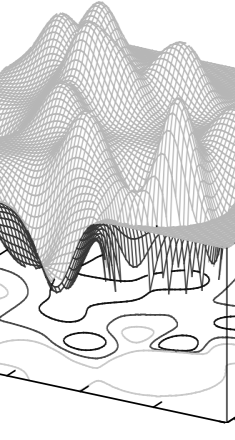
\includegraphics[height=7cm]{classPicture2-bw}
    }{\center

      \textbf{\fontsize{17}{20}\selectfont \course}

      ~

      %Lecture
      \topic\\

      \vspace{1cm}

      {\tiny~\emph{\keywords}~\\}

      \vspace{1cm}

      Marc Toussaint
      
      University of Stuttgart

      Summer 2019

      ~

    }
  }
}

\newcommand{\slide}[2]{
  \slidefont
  \incpage\begin{frame}
  \addcontentsline{toc}{section}{#1}
  \vfill
  {\headerfont #1} \vspace*{-2ex}
  \begin{itemize}\item[]~\\
    #2
  \end{itemize}
  \vfill
  \end{frame}
}

\newenvironment{slidecore}[1]{
  \slidefont\incpage
  \addcontentsline{toc}{section}{#1}
  \vfill
  {\headerfont #1} \vspace*{-2ex}
  \begin{itemize}\item[]~\\
}{
  \end{itemize}
  \vfill
}


\providecommand{\key}[1]{
  \addtocounter{mypage}{1}
% \immediate\write\keyfile{#1}
  \addtocontents{toc}{\hyperref[key:#1]{#1 (\arabic{mypage})}}
%  \phantomsection\label{key:#1}
%  \index{#1@{\hyperref[key:#1]{#1 (\arabic{mysec}:\arabic{mypage})}}|phantom}
  \addtocounter{mypage}{-1}
}

\providecommand{\course}{}

\providecommand{\subtopic}{}

\providecommand{\sublecture}[2]{
  \renewcommand{\subtopic}{#1}
  \slide{#1}{#2}
}

\providecommand{\story}[1]{
~

Motivation: {\tiny #1}\clearpage
}

\newenvironment{items}[1][9]{
\par\setlength{\unitlength}{1pt}\fontsize{#1}{#1}\linespread{1.2}\selectfont
\begin{list}{--}{\leftmargin4ex \rightmargin0ex \labelsep1ex \labelwidth2ex
\topsep0pt \parsep0ex \itemsep3pt}
}{
\end{list}
}

\providecommand{\slidesfoot}{
  \end{document}
}


  \slideshead
}

\providecommand{\exercises}{
  \newcommand{\exerciseshead}{
  \documentclass[10pt,fleqn]{article}
  \stdpackages

  \definecolor{bluecol}{rgb}{0,0,.5}
  \definecolor{greencol}{rgb}{0,.4,0}
  \definecolor{shadecolor}{gray}{0.9}
  \usepackage[
    %    pdftex%,
    %%    letterpaper,
    %    bookmarks,
    %    bookmarksnumbered,
    colorlinks,
    urlcolor=bluecol,
    citecolor=black,
    linkcolor=bluecol,
    %    pagecolor=bluecol,
    pdfborder={0 0 0},
    %pdfborderstyle={/S/U/W 1},
    %%    backref,     %link from bibliography back to sections
    %%    pagebackref, %link from bibliography back to pages
    %%    pdfstartview=FitH, %fitwidth instead of fit window
    pdfpagemode=UseNone, %UseOutlines, %bookmarks are displayed by acrobat
    pdftitle={\course},
    pdfauthor={Marc Toussaint},
    pdfkeywords={}
  ]{hyperref}
  \DeclareGraphicsExtensions{.pdf,.png,.jpg,.eps}

  \renewcommand{\r}{\varrho}
  \renewcommand{\l}{\lambda}
  \renewcommand{\L}{\Lambda}
  \renewcommand{\b}{\beta}
  \renewcommand{\d}{\delta}
  \renewcommand{\k}{\kappa}
  \renewcommand{\t}{\theta}
  \renewcommand{\O}{\Omega}
  \renewcommand{\o}{\omega}
  \renewcommand{\SS}{{\cal S}}
  \renewcommand{\=}{\!=\!}
  %\renewcommand{\boldsymbol}{}
  %\renewcommand{\Chapter}{\chapter}
  %\renewcommand{\Subsection}{\subsection}

  \renewcommand{\baselinestretch}{1.1}
  \geometry{a4paper,headsep=7mm,hdivide={15mm,*,15mm},vdivide={20mm,*,15mm}}

  \fancyhead[L]{\thetitle, \textit{Marc Toussaint}---\today}
  \fancyhead[R]{\thepage}
  \fancyhead[C]{}
  \fancyfoot{}
  \pagestyle{fancy}

  \parindent 0pt
  \parskip 0.5ex

  \newcommand{\codefont}{\helvetica{8}{1.2}{m}{n}}

  %auto-ignore
  \renewcommand{\a}{\alpha}
  \renewcommand{\b}{\beta}
  \renewcommand{\d}{\delta}
    \newcommand{\D}{\Delta}
    \newcommand{\e}{\epsilon}
    \newcommand{\g}{\gamma}
    \newcommand{\G}{\Gamma}
  \renewcommand{\l}{\lambda}
  \renewcommand{\L}{\Lambda}
    \newcommand{\m}{\mu}
    \newcommand{\n}{\nu}
    \newcommand{\N}{\nabla}
  \renewcommand{\k}{\kappa}
  \renewcommand{\o}{\omega}
  \renewcommand{\O}{\Omega}
    \newcommand{\p}{\phi}
    \newcommand{\ph}{\varphi}
  \renewcommand{\P}{\Phi}
  \renewcommand{\r}{\varrho}
    \newcommand{\s}{\sigma}
  \renewcommand{\S}{\Sigma}
  \renewcommand{\t}{\theta}
    \newcommand{\T}{\Theta}
  %\renewcommand{\v}{\vartheta}
    \newcommand{\x}{\xi}
    \newcommand{\X}{\Xi}
    \newcommand{\Y}{\Upsilon}
    \newcommand{\z}{\zeta}

  \renewcommand{\AA}{{\cal A}}
    \newcommand{\BB}{{\cal B}}
    \newcommand{\CC}{{\cal C}}
    \newcommand{\cc}{{\cal c}}
    \newcommand{\DD}{{\cal D}}
    \newcommand{\EE}{{\cal E}}
    \newcommand{\FF}{{\cal F}}
    \newcommand{\GG}{{\cal G}}
    \newcommand{\HH}{{\cal H}}
    \newcommand{\II}{{\cal I}}
    \newcommand{\KK}{{\cal K}}
    \newcommand{\LL}{{\cal L}}
    \newcommand{\MM}{{\cal M}}
    \newcommand{\NN}{{\cal N}}
    \newcommand{\oNN}{\overline\NN}
    \newcommand{\OO}{{\cal O}}
    \newcommand{\PP}{{\cal P}}
    \newcommand{\QQ}{{\cal Q}}
    \newcommand{\RR}{{\cal R}}
  \renewcommand{\SS}{{\cal S}}
    \newcommand{\TT}{{\cal T}}
    \newcommand{\uu}{{\cal u}}
    \newcommand{\UU}{{\cal U}}
    \newcommand{\VV}{{\cal V}}
    \newcommand{\XX}{{\cal X}}
    \newcommand{\xx}{\mathcal{x}}
    \newcommand{\YY}{{\cal Y}}
    \newcommand{\SOSO}{{\cal SO}}
    \newcommand{\GLGL}{{\cal GL}}

    \newcommand{\Ee}{{\rm E}}

  \newcommand{\NNN}{{\mathbb{N}}}
  \newcommand{\III}{{\mathbb{I}}}
  \newcommand{\ZZZ}{{\mathbb{Z}}}
  %\newcommand{\RRR}{{\mathrm{I\!R}}}
  \newcommand{\RRR}{{\mathbb{R}}}
  \newcommand{\SSS}{{\mathbb{S}}}
  \newcommand{\CCC}{{\mathbb{C}}}
  \newcommand{\DDD}{{\mathbb{D}}}
  \newcommand{\one}{{{\bf 1}}}
  \newcommand{\eee}{\text{e}}

  \newcommand{\NNNN}{{\overline{\cal N}}}

  \renewcommand{\[}{\Big[}
  \renewcommand{\]}{\Big]}
  \renewcommand{\(}{\Big(}
  \renewcommand{\)}{\Big)}
  \renewcommand{\|}{\,|\,}
  \renewcommand{\;}{\,;\,}
  \renewcommand{\=}{\!=\!}
    \newcommand{\<}{\left\langle}
  \renewcommand{\>}{\right\rangle}

  \newcommand{\na}[1][]{{\nabla_{\!\!#1}}}
  \newcommand{\he}[1][]{{\nabla_{\!\!#1}^2}}
  \newcommand{\Prob}{{\rm Prob}}
  \newcommand{\Dir}{{\rm Dir}}
  \newcommand{\Beta}{{\rm Beta}}
  \newcommand{\Bern}{{\rm Bern}}
  \newcommand{\Bin}{{\rm Bin}}
  \newcommand{\Mult}{{\rm Mult}}
  \newcommand{\Aut}{{\rm Aut}}
  \newcommand{\cor}{{\rm cor}}
  \newcommand{\corr}{{\rm corr}}
  \newcommand{\sd}{{\rm sd}}
  \newcommand{\tr}{{\rm tr}}
  \newcommand{\Tr}{{\rm Tr}}
  \newcommand{\rank}{{\rm rank}}
  \newcommand{\diag}{{\rm diag}}
  \newcommand{\dom}{{\rm dom}}
  \newcommand{\id}{{\rm id}}
  \newcommand{\Id}{{\rm\bf I}}
  \newcommand{\Gl}{{\rm Gl}}
  \renewcommand{\th}{\ensuremath{{}^\text{th}} }
  \newcommand{\lag}{\mathcal{L}}
  \newcommand{\inn}{\rfloor}
  \newcommand{\lie}{\pounds}
  \newcommand{\longto}{\longrightarrow}
  \newcommand{\speer}{\parbox{0.4ex}{\raisebox{0.8ex}{$\nearrow$}}}
  \renewcommand{\dag}{ {}^\dagger }
  \newcommand{\blbox}{\rule{1ex}{1ex}}
  \newcommand{\Ji}{J^\sharp}
  \newcommand{\h}{{}^\star}
  \newcommand{\w}{\wedge}
  \newcommand{\too}{\longrightarrow}
  \newcommand{\oot}{\longleftarrow}
  \newcommand{\To}{\Rightarrow}
  \newcommand{\oT}{\Leftarrow}
  \newcommand{\oTo}{\Leftrightarrow}
  \renewcommand{\iff}{~\Longleftrightarrow~}
  \newcommand{\Too}{\;\Longrightarrow\;}
  \newcommand{\oto}{\leftrightarrow}
  \newcommand{\ot}{\leftarrow}
  \newcommand{\ootoo}{\longleftrightarrow}
  \newcommand{\ow}{\stackrel{\circ}\wedge}
  \newcommand{\defeq}{\stackrel{\hspace{0.2ex}{}_\Delta}=}
%  \newcommand{\defeq}{{\overstack\Delta =}}
  \newcommand{\feed}{\nonumber \\}
  \newcommand{\comma}{~,\quad}
  \newcommand{\period}{~.\quad}
  \newcommand{\del}{\partial}
%  \newcommand{\quabla}{\Delta}
  \newcommand{\point}{$\bullet~~$}
  \newcommand{\doubletilde}{ ~ \raisebox{0.3ex}{$\widetilde {}$} \raisebox{0.6ex}{$\widetilde {}$} \!\! }
  \newcommand{\topcirc}{\parbox{0ex}{~\raisebox{2.5ex}{${}^\circ$}}}
  \newcommand{\topdot} {\parbox{0ex}{~\raisebox{2.5ex}{$\cdot$}}}
  \newcommand{\topddot} {\parbox{0ex}{~\raisebox{1.3ex}{$\ddot{~}$}}}
  \newcommand{\sym}{\topcirc}
  \newcommand{\tsum}{\textstyle\sum}
  \newcommand{\st}{\quad\text{s.t.}\quad}

  \newcommand{\half}{\ensuremath{\frac{1}{2}}}
  \newcommand{\third}{\ensuremath{\frac{1}{3}}}
  \newcommand{\fourth}{\ensuremath{\frac{1}{4}}}

  \newcommand{\ubar}{\underline}
  %\renewcommand{\vec}{\underline}
  \renewcommand{\vec}{\boldsymbol}
  %\renewcommand{\_}{\underset}
  %\renewcommand{\^}{\overset}
  %\renewcommand{\*}{{\rm\raisebox{-.6ex}{\text{*}}{}}}
  \renewcommand{\*}{\text{\footnotesize\raisebox{-.4ex}{*}{}}}

  \newcommand{\gto}{{\raisebox{.5ex}{${}_\rightarrow$}}}
  \newcommand{\gfrom}{{\raisebox{.5ex}{${}_\leftarrow$}}}
  \newcommand{\gnto}{{\raisebox{.5ex}{${}_\nrightarrow$}}}
  \newcommand{\gnfrom}{{\raisebox{.5ex}{${}_\nleftarrow$}}}

  %\newcommand{\RND}{{\SS}}
  %\newcommand{\IF}{\text{if }}
  %\newcommand{\AND}{\textsc{and }}
  %\newcommand{\OR}{\textsc{or }}
  %\newcommand{\XOR}{\textsc{xor }}
  %\newcommand{\NOT}{\textsc{not }}

  %\newcommand{\argmax}[1]{{\rm arg}\!\max_{#1}}
  %\newcommand{\argmin}[1]{{\rm arg}\!\min_{#1}}
  \DeclareMathOperator*{\argmax}{argmax}
  \DeclareMathOperator*{\argmin}{argmin}
  \DeclareMathOperator{\sign}{sign}
  \DeclareMathOperator{\acos}{acos}
  \DeclareMathOperator{\unifies}{unifies}
  \DeclareMathOperator{\Span}{span}
  \newcommand{\ortho}{\perp}
  %\newcommand{\argmax}[1]{\underset{~#1}{\text{argmax}}\;}
  %\newcommand{\argmin}[1]{\underset{~#1}{\text{argmin}}\;}
  \newcommand{\ee}[1]{\ensuremath{\cdot10^{#1}}}
  \newcommand{\sub}[1]{\ensuremath{_{\text{#1}}}}
  \newcommand{\up}[1]{\ensuremath{^{\text{#1}}}}
  \newcommand{\kld}[3][{}]{D_{#1}\big(#2\,\big|\!\big|\,#3\big)}
  %\newcommand{\kld}[2]{D\big(#1:#2\big)}
  \newcommand{\sprod}[2]{\big<#1\,,\,#2\big>}
  \newcommand{\End}{\text{End}}
  \newcommand{\txt}[1]{\quad\text{#1}\quad}
  \newcommand{\Over}[2]{\genfrac{}{}{0pt}{0}{#1}{#2}}
  %\newcommand{\mat}[1]{{\bf #1}}
  \newcommand{\arr}[2]{\hspace*{-.5ex}\begin{array}{#1}#2\end{array}\hspace*{-.5ex}}
  \newcommand{\mat}[3][.9]{
    \renewcommand{\arraystretch}{#1}{\scriptscriptstyle{\left(
      \hspace*{-1ex}\begin{array}{#2}#3\end{array}\hspace*{-1ex}
    \right)}}\renewcommand{\arraystretch}{1.2}
  }
  \newcommand{\Mat}[3][.9]{
    \renewcommand{\arraystretch}{#1}{\scriptscriptstyle{\left[
      \hspace*{-1ex}\begin{array}{#2}#3\end{array}\hspace*{-1ex}
    \right]}}\renewcommand{\arraystretch}{1.2}
  }
  \newcommand{\case}[2][ll]{\left\{\arr{#1}{#2}\right.}
  \newcommand{\seq}[1]{\textsf{\<#1\>}}
  \newcommand{\seqq}[1]{\textsf{#1}}
  \newcommand{\floor}[1]{\lfloor#1\rfloor}
  \newcommand{\Exp}[2][]{\text{E}_{#1}\{#2\}}
  \newcommand{\Var}[2][]{\text{Var}_{#1}\{#2\}}
  \newcommand{\cov}[2][]{\text{cov}_{#1}\{#2\}}

  %\newcommand{\Exp}[2]{\left\langle{#2}\right\rangle_{#1}}
  \newcommand{\ex}{\setminus}

  \providecommand{\href}[2]{{\color{blue}USE PDFLATEX!}}
  \providecommand{\url}[2]{\href{#1}{{\color{blue}#2}}}
%  \newcommand{\link}[1]{\href{{\protect #1}}{\texttt{\protect #1}}}
  \newcommand{\anchor}[2]{\begin{picture}(0,0)\put(#1){#2}\end{picture}}
  \newcommand{\pagebox}{\begin{picture}(0,0)\put(-3,-23){
    \textcolor[rgb]{.5,1,.5}{\framebox[\textwidth]{\rule[-\textheight]{0pt}{0pt}}}}
    \end{picture}}

  \newcommand{\hide}[1]{
    \begin{list}{}{\leftmargin0ex \rightmargin0ex \topsep0ex \parsep0ex}
       \helvetica{5}{1}{m}{n}
       \renewcommand{\section}{\par SECTION: }
       \renewcommand{\subsection}{\par SUBSECTION: }
       \item[$~~\blacktriangleright$]
       #1%$\blacktriangleleft~~$
       \message{^^JHIDE--Warning!^^J}
    \end{list}
  }
  %\newcommand{\hide}[1]{{\tt[hide:~}{\footnotesize\sf #1}{\tt]}\message{^^JHIDE--Warning!^^J}}
  \newcommand{\Hide}{\renewcommand{\hide}[1]{\message{^^JHIDE--Warning (hidden)!^^J}}}
  \newcommand{\HIDE}{\renewcommand{\hide}[1]{}}
  \newcommand{\fullhide}[1]{\message{^^JHIDE--Warning (hidden)!^^J}}
  \newcommand{\todo}[1]{{\tt[TODO: #1]}\message{^^JTODO--Warning: #1^^J}}
  \newcommand{\Todo}{\renewcommand{\todo}[1]{\message{^^JTODO--Warning (hidden)!^^J}}}
  %\renewcommand{\title}[1]{\renewcommand{\thetitle}{#1}}
  \newcommand{\myauthor}[1]{\author{#1}\newcommand{\theauthor}{#1}}%\@author}
  \newcommand{\mytitle}[1]{\title{#1}\newcommand{\thetitle}{#1}}%\@title}
  \newcommand{\header}{\begin{document}\mytitle\cleardefs}
  \newcommand{\contents}{{\tableofcontents}\renewcommand{\contents}{}}
  \newcommand{\footer}{\small\bibliography{marc,bibs}\end{document}}
  \newcommand{\widepaper}{\usepackage{geometry}\geometry{a4paper,hdivide={25mm,*,25mm},vdivide={25mm,*,25mm}}}
  \newcommand{\moviex}[2]{\movie[externalviewer]{#1}{#2}} %\pdflatex\usepackage{multimedia}
  \newcommand{\rbox}[1]{\fboxrule2mm\fcolorbox[rgb]{1,.85,.85}{1,.85,.85}{#1}}
  \newcommand{\mpage}[2]{{\begin{minipage}{#1\columnwidth}#2\end{minipage}}}
  \newcommand{\redbox}[2]{\fboxrule1mm\fcolorbox[rgb]{1,.7,.7}{1,.7,.7}{\begin{minipage}{#1\columnwidth}\center#2\end{minipage}}}
  \newcommand{\onecol}[2]{
    \begin{minipage}[c]{#1\columnwidth}#2\end{minipage}}
  \newcommand{\twocol}[5][0]{
    \begin{minipage}[c]{#2\columnwidth}#4\end{minipage}\hspace*{#1\columnwidth}%
    \begin{minipage}[c]{#3\columnwidth}#5\end{minipage}}
  \newcommand{\threecol}[7][0]{%
    \begin{minipage}[c]{#2\columnwidth}#5\end{minipage}\hspace*{#1\columnwidth}%
    \begin{minipage}[c]{#3\columnwidth}#6\end{minipage}\hspace*{#1\columnwidth}%
    \begin{minipage}[c]{#4\columnwidth}#7\end{minipage}}
  \newcommand{\threecoltext}[7][c]{
    \begin{minipage}[#1]{#2\textwidth}#5\end{minipage}%
    \begin{minipage}[#1]{#3\textwidth}#6\end{minipage}%
    \begin{minipage}[#1]{#4\textwidth}#7\end{minipage}}
  \newcommand{\threecoltop}[7][0]{%
   \begin{minipage}[t]{#2\columnwidth}#5\end{minipage}\hspace*{#1\columnwidth}%
   \begin{minipage}[t]{#3\columnwidth}#6\end{minipage}\hspace*{#1\columnwidth}%
   \begin{minipage}[t]{#4\columnwidth}#7\end{minipage}}
  \newcommand{\fourcol}[9][0]{%
   \begin{minipage}[c]{#2\columnwidth}#6\end{minipage}\hspace*{#1\columnwidth}%
   \begin{minipage}[c]{#3\columnwidth}#7\end{minipage}\hspace*{#1\columnwidth}%
   \begin{minipage}[c]{#4\columnwidth}#8\end{minipage}\hspace*{#1\columnwidth}%
   \begin{minipage}[c]{#5\columnwidth}#9\end{minipage}}
  \newcommand{\helvetica}[4]{\setlength{\unitlength}{1pt}\fontsize{#1}{#1}\linespread{#2}\usefont{OT1}{phv}{#3}{#4}}
  \newcommand{\helve}[1]{\helvetica{#1}{1.5}{m}{n}}
  \newcommand{\german}{\usepackage[german]{babel}\usepackage[utf8]{inputenc}}

\newcommand{\norm}[1]{|\!|#1|\!|}
\newcommand{\expr}[1]{[\hspace{-.2ex}[#1]\hspace{-.2ex}]}

\newcommand{\Jwi}{J^\sharp_W}
\newcommand{\THi}{T^\sharp_H}
\newcommand{\Jci}{J^\natural_C}
\newcommand{\hJi}{{\bar J}^\sharp}
\renewcommand{\|}{\,|\,}
\renewcommand{\=}{\!=\!}
\newcommand{\myminus}{{\hspace*{-.0pt}\text{\rm -}\hspace*{-.5pt}}}
\newcommand{\myplus}{{\hspace*{-.0pt}\text{\rm +}\hspace*{-.5pt}}}
\newcommand{\1}{{\myminus1}}
\newcommand{\2}{{\myminus2}}
\newcommand{\3}{{\myminus3}}
\newcommand{\mT}{{\text{\rm -}\hspace*{-1pt}\top}}
\newcommand{\po}{{\myplus1}}
\newcommand{\pt}{{\myplus2}}
%\renewcommand{\-}{\myminus}
%\newcommand{\+}{\myplus}
\renewcommand{\T}{{\!\top\!}}
\newcommand{\xT}{{\underline x}}
\newcommand{\uT}{{\underline u}}
\newcommand{\zT}{{\underline z}}
\newcommand{\Sum}{\textstyle\sum}
\newcommand{\Int}{\textstyle\int}
\newcommand{\Prod}{\textstyle\prod}


\newenvironment{centy}{
\vspace{15mm}
\large
\hspace*{5mm}
\begin{minipage}{8cm}\it\color{blue}
}{
\end{minipage}
}

\newcommand{\old}{{\text{old}}}
\newcommand{\new}{{\text{new}}}
\newcommand{\MAP}{{\text{MAP}}}
\newcommand{\ML}{{\text{ML}}}

\newcommand{\redArrow}{\quad\anchor{0,-1}{\includegraphics[scale=.5]{figs/redArrow}}}
\newcommand{\pub}[1]{{\color{green}\helvetica{8}{1.3}{m}{n}#1\\}}
\DeclareMathOperator{\opKL}{KL}
\newcommand{\KL}[2]{\opKL\big(#1\,\big|\!\big|\,#2\big)} %\left(#1 |\!| #2\right)}

\renewcommand{\show}[2][.8]{\centerline{\includegraphics[width=#1\columnwidth]{#2}}}
\newcommand{\showh}[2][.8]{\includegraphics[width=#1\columnwidth]{#2}}
\newcommand{\shows}[2][.8]{\centerline{\includegraphics[scale=#1]{#2}}}
\newcommand{\showhs}[2][.8]{\includegraphics[scale=#1]{#2}}
\newcommand{\mov}[2]{\movie[externalviewer]{{\color{blue}\small #1}}{movies/#2}}
\newcommand{\movex}[2]{\movie[externalviewer]{#1}{#2}} %\pdflatex\usepackage{multimedia}
%\newcommand{\movgb}[1]{\hfill\movie[externalviewer]{\small[movie]}{/home/mtoussai/movies/10-goalDirectedBehavior/#1}}
\newcommand{\movh}[3][loop]{
\movie[#1]{\showh[#2]{movies/#3.png}}{movies/#3.avi}%
\movie[externalviewer]{$\circ$}{movies/#3.avi}
}
\newcommand{\movc}[3][loop]{\centerline{\movh[#1]{#2}{#3}}}
\newcommand{\cen}[1]{\centerline{#1}}

\newcommand{\citing}[1]{
{\color{citcol}\tiny#1\par}
}

\newcommand{\cit}[3]{
\par\smallskip
{\color{greencol}\tiny #1: \emph{#2}. #3 \par}
}

\newcommand{\citurl}[4]{
\par\smallskip
{\color{greencol}\tiny #1: \protect{\href{#4}{\color{blue}{#2.}}} #3 \par}
}

\newcommand{\cito}[3]{
\par\smallskip
{\color{bluecol}\tiny #1: \emph{#2}. #3 \par}
}

\newcommand{\redoMacrosInProof}{
  \renewcommand{\d}{\delta}
%  \renewcommand{\|}{\,|\,}
  \renewcommand{\=}{\!=\!}
}

%% \makeatletter
%% \newenvironment{code}{%
%%   \begin{lrbox}{\@tempboxa}\begin{minipage}{1\columnwidth}\codefont
%% }{
%%   \end{minipage}\end{lrbox}%
%%   \colorbox[rgb]{.95,.95,.95}{\usebox{\@tempboxa}}
%% }\makeatother

\newenvironment{code}{%
\codefont
\begin{shaded}
}{
\end{shaded}
}

%\newcommand{\refeq}[1]{(\ref{#1})}

\usepackage{algorithm}
\usepackage{algpseudocode}
\algrenewcommand{\algorithmicrequire}{\textbf{Input:~~}}
\algrenewcommand{\algorithmicensure}{\textbf{Output:}}
\algrenewcommand{\algorithmiccomment}[1]{\qquad\hfill~\hspace*{-5ex}\textit{// #1}}
\algrenewcommand{\alglinenumber}[1]{\helvetica{6}{1.3}{m}{n}#1:}

\newenvironment{algo}[1][8]{
\quad\begin{minipage}{.8\columnwidth}\helvetica{#1}{1.3}{m}{n}
\medskip\hrule\medskip
\begin{algorithmic}[1]
}{
\end{algorithmic}
\medskip\hrule\medskip
\end{minipage}
}

\usepackage{etoolbox}

%%%%%%%%%%%%%%%%%%%%%%%%%%%%%%%%%%%%%%%%%%%%%%%%%%%%%%%%%%%%%%%%%%%%%%%%%%%%%%%%

\usepackage{multirow}
\usepackage{colortbl}
%\setlength{\jot}{0pt}
%\setlength{\mathindent}{1ex}
\usepackage{empheq}

%%%%%%%%%%%%%%%%%%%%%%%%%%%%%%%%%%%%%%%%%%%%%%%%%%%%%%%%%%%%%%%%%%%%%%%%%%%%%%%

\newcommand{\mypause}{\pause}
%\newcommand{\dom}{{\text{dom}}}
\newcommand{\defi}[1]{\textbf{#1}}
\newcommand{\red}[1]{\emph{\color{red}#1}}
%\newcommand{\ul}{\underline}
\newcommand{\pos}{{\textsf{pos}}}
\newcommand{\eff}{{\textsf{eff}}}
\newcommand{\rot}{{\textsf{rot}}}
\newcommand{\veC}{{\textsf{vec}}}
\newcommand{\quat}{{\textsf{quat}}}
\newcommand{\col}{{\textsf{col}}}
\newcommand{\de}[2]{\frac{\partial #1}{\partial #2}}
\newcommand{\target}{{\text{target}}}
\newcommand{\near}{{\text{near}}}
\newcommand{\qfree}{Q_{\text{free}}}
\renewcommand{\vec}{\boldsymbol}
\newcommand{\lft}{\text{left}}
\newcommand{\rgh}{\text{right}}
\DeclareMathOperator{\real}{real}
\newcommand{\prev}{{\text{prev}}}
\newcommand{\TR}[2]{T_{{#1}\shortrightarrow{#2}}}
\newcommand{\RO}[2]{R_{{#1}\shortrightarrow{#2}}}
\newcommand{\liter}{\helvetica{8}{1.1}{m}{n}\parskip 1ex}
\newcommand{\Fc}{\color{green}F}
\newcommand{\muc}{\color{blue}\mu}
\newcommand{\Astar}{A$^*$}

%for optimization course:
\newcommand{\adec}{\r_\a^-}
\newcommand{\ainc}{\r_\a^+}
\newcommand{\ldec}{\r_\l^-}
\newcommand{\linc}{\r_\l^+}
\newcommand{\minc}{\r_\m^+}
\newcommand{\mdec}{\r_\m^-}
\newcommand{\lsstop}{\r_{\text{ls}}}


\definecolor{boxcol}{rgb}{.85,.9,.92}
\newcommand{\eqbox}[1]{\centerline{\fboxrule0mm\fcolorbox{boxcol}{boxcol}{#1}}}
\newcommand{\movgb}[1]{\hfill\movie[externalviewer]{\small[movie]}{/home/mtoussai/movies/10-goalDirectedBehavior/#1}}
\newcommand{\demo}[1]{{{\color{blue}[\small #1]}}}

\graphicspath{{../pics-robotics/}{../pics-ML/}{../pics-all/}{../pics-all2/}{../pics-Optim/}}
\DeclareGraphicsExtensions{.pdf,.png,.jpg}

%\usepackage{pdfpages}
%\setbeamercolor{background canvas}{bg=}

\newcommand{\SUM}{\texttt{sum}}
\usepackage{float}

%% prevent pagebreaks before environment
\makeatletter
\newcommand{\NewParNoBreak}[1][\parskip]{\par\vspace*{-\parskip}\vspace*{#1}\nobreak\@afterheading}
\makeatother

%\newcommand{\idx}[2]{\label{IKgn}}

%%%%%%%%%%%%%%%%%%%%%%%%%%%%%%%%%%%%%%%%%%%%%%%%%%%%%%%%%%%%%%%%%%%%%%%%%%%%%%%%



%% \newwrite\tempfile
%% \immediate\openout\tempfile=z.keys.tex

%% \renewcommand{\key}[1]{
%% %%   \addtocounter{mypage}{1}
%% \makeatletter
%% \immediate\write\tempfile{\symbol{`\\}}
%% \makeatother
%%   \immediate\write\tempfile{hyperref[key:#1]{#1(\arabic{mypage})}}
%% %%  % \phantomsection\label{key:#1}
%% %%   %\index{#1@{\hyperref[key:#1]{#1 (\arabic{mysec}:\arabic{mypage})}}|phantom}
%% %%   \addtocounter{mypage}{-1}
%% }


  \DefineShortVerb{\@}

  \newcounter{solutions}
  \setcounter{solutions}{1}
  \newenvironment{solution}{
    \small
    \begin{shaded}
  }{
    \end{shaded}
  }
  
  \renewcommand{\hat}{\widehat}
  \newcommand{\bbg}{{\bar{\bar g}}}
  \graphicspath{{pics/}{../shared/pics/}}

  \renewcommand{\labelenumi}{{\alph{enumi})}}

  %%%%%%%%%%%%%%%%%%%%%%%%%%%%%%%%%%%%%%%%%%%%%%%%%%%%%%%%%%%%%%%%%%%%%%%%%%%%%%%%


  \mytitle{\course\\Exercise \exnum}
  \myauthor{Marc Toussaint\\ TAs: Janik Hager, Philipp Kratzer\\\small\addressUSTT}
  
  
  \begin{document}
  \onecolumn
  \maketitle
}

\newcommand{\exsection}[1]{\section{#1}}

\newcommand{\exerfoot}{
  \end{document}
}

\newenvironment{items}[1][9]{
  \par\setlength{\unitlength}{1pt}\fontsize{#1}{#1}\linespread{1.2}\selectfont
  \begin{list}{--}{\leftmargin4ex \rightmargin0ex \labelsep1ex \labelwidth2ex
      \topsep0pt \parsep0ex \itemsep3pt}
}{
  \end{list}
}

  \exerciseshead
}

\providecommand{\script}{
  \newcommand{\scripthead}{
  \documentclass[9pt,twoside]{article}
  \stdpackages

  \usepackage{palatino}
  \usepackage[envcountsect]{beamerarticle}
  \usepackage{makeidx}
  \makeindex

  \definecolor{bluecol}{rgb}{0,0,.5}
  \definecolor{greencol}{rgb}{0,.4,0}
  \definecolor{shadecolor}{gray}{0.9}
  \usepackage[
    %    pdftex%,
    %%    letterpaper,
    %bookmarks,
    bookmarksnumbered,
    colorlinks,
    urlcolor=bluecol,
    citecolor=black,
    linkcolor=bluecol,
    %    pagecolor=bluecol,
    pdfborder={0 0 0},
    %pdfborderstyle={/S/U/W 1},
    %%    backref,     %link from bibliography back to sections
    %%    pagebackref, %link from bibliography back to pages
    %%    pdfstartview=FitH, %fitwidth instead of fit window
    pdfpagemode=UseOutlines, %bookmarks are displayed by acrobat
    pdftitle={\course},
    pdfauthor={Marc Toussaint},
    pdfkeywords={}
  ]{hyperref}
  \DeclareGraphicsExtensions{.pdf,.png,.jpg,.eps}

  \usepackage{multimedia}
  %\setbeamercolor{background canvas}{bg=}

  \renewcommand{\r}{\varrho}
  \renewcommand{\l}{\lambda}
  \renewcommand{\L}{\Lambda}
  \renewcommand{\b}{\beta}
  \renewcommand{\d}{\delta}
  \renewcommand{\k}{\kappa}
  \renewcommand{\t}{\theta}
  \renewcommand{\O}{\Omega}
  \renewcommand{\o}{\omega}
  \renewcommand{\SS}{{\cal S}}
  \renewcommand{\=}{\!=\!}
  %\renewcommand{\boldsymbol}{}
  %\renewcommand{\Chapter}{\chapter}
  %\renewcommand{\Subsection}{\subsection}

  \renewcommand{\baselinestretch}{1.0}
  \geometry{a5paper,headsep=6mm,hdivide={10mm,*,10mm},vdivide={13mm,*,7mm}}

  \fancyhead[OL,ER]{\course, \textit{Marc Toussaint}}
  \fancyhead[OR,EL]{\thepage}
  \fancyhead[C]{}
  \fancyfoot{}
  \pagestyle{fancy}

%  \setcounter{tocdepth}{3}
  \setcounter{tocdepth}{2}

   \columnsep 6ex
  %  \renewcommand{\familydefault}{\sfdefault}
  \newcommand{\headerfont}{\large}%helvetica{12}{1}{b}{n}}
  \newcommand{\slidefont} {}%\helvetica{9}{1.3}{m}{n}}
  \newcommand{\storyfont} {}
  %  \renewcommand{\small}   {\helvetica{8}{1.2}{m}{n}}
  \renewcommand{\tiny}    {\footnotesize}%helvetica{7}{1.1}{m}{n}}
  \newcommand{\codefont}{\fontsize{6}{6}\selectfont}%helvetica{8}{1.2}{m}{n}}

  %auto-ignore
  \renewcommand{\a}{\alpha}
  \renewcommand{\b}{\beta}
  \renewcommand{\d}{\delta}
    \newcommand{\D}{\Delta}
    \newcommand{\e}{\epsilon}
    \newcommand{\g}{\gamma}
    \newcommand{\G}{\Gamma}
  \renewcommand{\l}{\lambda}
  \renewcommand{\L}{\Lambda}
    \newcommand{\m}{\mu}
    \newcommand{\n}{\nu}
    \newcommand{\N}{\nabla}
  \renewcommand{\k}{\kappa}
  \renewcommand{\o}{\omega}
  \renewcommand{\O}{\Omega}
    \newcommand{\p}{\phi}
    \newcommand{\ph}{\varphi}
  \renewcommand{\P}{\Phi}
  \renewcommand{\r}{\varrho}
    \newcommand{\s}{\sigma}
  \renewcommand{\S}{\Sigma}
  \renewcommand{\t}{\theta}
    \newcommand{\T}{\Theta}
  %\renewcommand{\v}{\vartheta}
    \newcommand{\x}{\xi}
    \newcommand{\X}{\Xi}
    \newcommand{\Y}{\Upsilon}
    \newcommand{\z}{\zeta}

  \renewcommand{\AA}{{\cal A}}
    \newcommand{\BB}{{\cal B}}
    \newcommand{\CC}{{\cal C}}
    \newcommand{\cc}{{\cal c}}
    \newcommand{\DD}{{\cal D}}
    \newcommand{\EE}{{\cal E}}
    \newcommand{\FF}{{\cal F}}
    \newcommand{\GG}{{\cal G}}
    \newcommand{\HH}{{\cal H}}
    \newcommand{\II}{{\cal I}}
    \newcommand{\KK}{{\cal K}}
    \newcommand{\LL}{{\cal L}}
    \newcommand{\MM}{{\cal M}}
    \newcommand{\NN}{{\cal N}}
    \newcommand{\oNN}{\overline\NN}
    \newcommand{\OO}{{\cal O}}
    \newcommand{\PP}{{\cal P}}
    \newcommand{\QQ}{{\cal Q}}
    \newcommand{\RR}{{\cal R}}
  \renewcommand{\SS}{{\cal S}}
    \newcommand{\TT}{{\cal T}}
    \newcommand{\uu}{{\cal u}}
    \newcommand{\UU}{{\cal U}}
    \newcommand{\VV}{{\cal V}}
    \newcommand{\XX}{{\cal X}}
    \newcommand{\xx}{\mathcal{x}}
    \newcommand{\YY}{{\cal Y}}
    \newcommand{\SOSO}{{\cal SO}}
    \newcommand{\GLGL}{{\cal GL}}

    \newcommand{\Ee}{{\rm E}}

  \newcommand{\NNN}{{\mathbb{N}}}
  \newcommand{\III}{{\mathbb{I}}}
  \newcommand{\ZZZ}{{\mathbb{Z}}}
  %\newcommand{\RRR}{{\mathrm{I\!R}}}
  \newcommand{\RRR}{{\mathbb{R}}}
  \newcommand{\SSS}{{\mathbb{S}}}
  \newcommand{\CCC}{{\mathbb{C}}}
  \newcommand{\DDD}{{\mathbb{D}}}
  \newcommand{\one}{{{\bf 1}}}
  \newcommand{\eee}{\text{e}}

  \newcommand{\NNNN}{{\overline{\cal N}}}

  \renewcommand{\[}{\Big[}
  \renewcommand{\]}{\Big]}
  \renewcommand{\(}{\Big(}
  \renewcommand{\)}{\Big)}
  \renewcommand{\|}{\,|\,}
  \renewcommand{\;}{\,;\,}
  \renewcommand{\=}{\!=\!}
    \newcommand{\<}{\left\langle}
  \renewcommand{\>}{\right\rangle}

  \newcommand{\na}[1][]{{\nabla_{\!\!#1}}}
  \newcommand{\he}[1][]{{\nabla_{\!\!#1}^2}}
  \newcommand{\Prob}{{\rm Prob}}
  \newcommand{\Dir}{{\rm Dir}}
  \newcommand{\Beta}{{\rm Beta}}
  \newcommand{\Bern}{{\rm Bern}}
  \newcommand{\Bin}{{\rm Bin}}
  \newcommand{\Mult}{{\rm Mult}}
  \newcommand{\Aut}{{\rm Aut}}
  \newcommand{\cor}{{\rm cor}}
  \newcommand{\corr}{{\rm corr}}
  \newcommand{\sd}{{\rm sd}}
  \newcommand{\tr}{{\rm tr}}
  \newcommand{\Tr}{{\rm Tr}}
  \newcommand{\rank}{{\rm rank}}
  \newcommand{\diag}{{\rm diag}}
  \newcommand{\dom}{{\rm dom}}
  \newcommand{\id}{{\rm id}}
  \newcommand{\Id}{{\rm\bf I}}
  \newcommand{\Gl}{{\rm Gl}}
  \renewcommand{\th}{\ensuremath{{}^\text{th}} }
  \newcommand{\lag}{\mathcal{L}}
  \newcommand{\inn}{\rfloor}
  \newcommand{\lie}{\pounds}
  \newcommand{\longto}{\longrightarrow}
  \newcommand{\speer}{\parbox{0.4ex}{\raisebox{0.8ex}{$\nearrow$}}}
  \renewcommand{\dag}{ {}^\dagger }
  \newcommand{\blbox}{\rule{1ex}{1ex}}
  \newcommand{\Ji}{J^\sharp}
  \newcommand{\h}{{}^\star}
  \newcommand{\w}{\wedge}
  \newcommand{\too}{\longrightarrow}
  \newcommand{\oot}{\longleftarrow}
  \newcommand{\To}{\Rightarrow}
  \newcommand{\oT}{\Leftarrow}
  \newcommand{\oTo}{\Leftrightarrow}
  \renewcommand{\iff}{~\Longleftrightarrow~}
  \newcommand{\Too}{\;\Longrightarrow\;}
  \newcommand{\oto}{\leftrightarrow}
  \newcommand{\ot}{\leftarrow}
  \newcommand{\ootoo}{\longleftrightarrow}
  \newcommand{\ow}{\stackrel{\circ}\wedge}
  \newcommand{\defeq}{\stackrel{\hspace{0.2ex}{}_\Delta}=}
%  \newcommand{\defeq}{{\overstack\Delta =}}
  \newcommand{\feed}{\nonumber \\}
  \newcommand{\comma}{~,\quad}
  \newcommand{\period}{~.\quad}
  \newcommand{\del}{\partial}
%  \newcommand{\quabla}{\Delta}
  \newcommand{\point}{$\bullet~~$}
  \newcommand{\doubletilde}{ ~ \raisebox{0.3ex}{$\widetilde {}$} \raisebox{0.6ex}{$\widetilde {}$} \!\! }
  \newcommand{\topcirc}{\parbox{0ex}{~\raisebox{2.5ex}{${}^\circ$}}}
  \newcommand{\topdot} {\parbox{0ex}{~\raisebox{2.5ex}{$\cdot$}}}
  \newcommand{\topddot} {\parbox{0ex}{~\raisebox{1.3ex}{$\ddot{~}$}}}
  \newcommand{\sym}{\topcirc}
  \newcommand{\tsum}{\textstyle\sum}
  \newcommand{\st}{\quad\text{s.t.}\quad}

  \newcommand{\half}{\ensuremath{\frac{1}{2}}}
  \newcommand{\third}{\ensuremath{\frac{1}{3}}}
  \newcommand{\fourth}{\ensuremath{\frac{1}{4}}}

  \newcommand{\ubar}{\underline}
  %\renewcommand{\vec}{\underline}
  \renewcommand{\vec}{\boldsymbol}
  %\renewcommand{\_}{\underset}
  %\renewcommand{\^}{\overset}
  %\renewcommand{\*}{{\rm\raisebox{-.6ex}{\text{*}}{}}}
  \renewcommand{\*}{\text{\footnotesize\raisebox{-.4ex}{*}{}}}

  \newcommand{\gto}{{\raisebox{.5ex}{${}_\rightarrow$}}}
  \newcommand{\gfrom}{{\raisebox{.5ex}{${}_\leftarrow$}}}
  \newcommand{\gnto}{{\raisebox{.5ex}{${}_\nrightarrow$}}}
  \newcommand{\gnfrom}{{\raisebox{.5ex}{${}_\nleftarrow$}}}

  %\newcommand{\RND}{{\SS}}
  %\newcommand{\IF}{\text{if }}
  %\newcommand{\AND}{\textsc{and }}
  %\newcommand{\OR}{\textsc{or }}
  %\newcommand{\XOR}{\textsc{xor }}
  %\newcommand{\NOT}{\textsc{not }}

  %\newcommand{\argmax}[1]{{\rm arg}\!\max_{#1}}
  %\newcommand{\argmin}[1]{{\rm arg}\!\min_{#1}}
  \DeclareMathOperator*{\argmax}{argmax}
  \DeclareMathOperator*{\argmin}{argmin}
  \DeclareMathOperator{\sign}{sign}
  \DeclareMathOperator{\acos}{acos}
  \DeclareMathOperator{\unifies}{unifies}
  \DeclareMathOperator{\Span}{span}
  \newcommand{\ortho}{\perp}
  %\newcommand{\argmax}[1]{\underset{~#1}{\text{argmax}}\;}
  %\newcommand{\argmin}[1]{\underset{~#1}{\text{argmin}}\;}
  \newcommand{\ee}[1]{\ensuremath{\cdot10^{#1}}}
  \newcommand{\sub}[1]{\ensuremath{_{\text{#1}}}}
  \newcommand{\up}[1]{\ensuremath{^{\text{#1}}}}
  \newcommand{\kld}[3][{}]{D_{#1}\big(#2\,\big|\!\big|\,#3\big)}
  %\newcommand{\kld}[2]{D\big(#1:#2\big)}
  \newcommand{\sprod}[2]{\big<#1\,,\,#2\big>}
  \newcommand{\End}{\text{End}}
  \newcommand{\txt}[1]{\quad\text{#1}\quad}
  \newcommand{\Over}[2]{\genfrac{}{}{0pt}{0}{#1}{#2}}
  %\newcommand{\mat}[1]{{\bf #1}}
  \newcommand{\arr}[2]{\hspace*{-.5ex}\begin{array}{#1}#2\end{array}\hspace*{-.5ex}}
  \newcommand{\mat}[3][.9]{
    \renewcommand{\arraystretch}{#1}{\scriptscriptstyle{\left(
      \hspace*{-1ex}\begin{array}{#2}#3\end{array}\hspace*{-1ex}
    \right)}}\renewcommand{\arraystretch}{1.2}
  }
  \newcommand{\Mat}[3][.9]{
    \renewcommand{\arraystretch}{#1}{\scriptscriptstyle{\left[
      \hspace*{-1ex}\begin{array}{#2}#3\end{array}\hspace*{-1ex}
    \right]}}\renewcommand{\arraystretch}{1.2}
  }
  \newcommand{\case}[2][ll]{\left\{\arr{#1}{#2}\right.}
  \newcommand{\seq}[1]{\textsf{\<#1\>}}
  \newcommand{\seqq}[1]{\textsf{#1}}
  \newcommand{\floor}[1]{\lfloor#1\rfloor}
  \newcommand{\Exp}[2][]{\text{E}_{#1}\{#2\}}
  \newcommand{\Var}[2][]{\text{Var}_{#1}\{#2\}}
  \newcommand{\cov}[2][]{\text{cov}_{#1}\{#2\}}

  %\newcommand{\Exp}[2]{\left\langle{#2}\right\rangle_{#1}}
  \newcommand{\ex}{\setminus}

  \providecommand{\href}[2]{{\color{blue}USE PDFLATEX!}}
  \providecommand{\url}[2]{\href{#1}{{\color{blue}#2}}}
%  \newcommand{\link}[1]{\href{{\protect #1}}{\texttt{\protect #1}}}
  \newcommand{\anchor}[2]{\begin{picture}(0,0)\put(#1){#2}\end{picture}}
  \newcommand{\pagebox}{\begin{picture}(0,0)\put(-3,-23){
    \textcolor[rgb]{.5,1,.5}{\framebox[\textwidth]{\rule[-\textheight]{0pt}{0pt}}}}
    \end{picture}}

  \newcommand{\hide}[1]{
    \begin{list}{}{\leftmargin0ex \rightmargin0ex \topsep0ex \parsep0ex}
       \helvetica{5}{1}{m}{n}
       \renewcommand{\section}{\par SECTION: }
       \renewcommand{\subsection}{\par SUBSECTION: }
       \item[$~~\blacktriangleright$]
       #1%$\blacktriangleleft~~$
       \message{^^JHIDE--Warning!^^J}
    \end{list}
  }
  %\newcommand{\hide}[1]{{\tt[hide:~}{\footnotesize\sf #1}{\tt]}\message{^^JHIDE--Warning!^^J}}
  \newcommand{\Hide}{\renewcommand{\hide}[1]{\message{^^JHIDE--Warning (hidden)!^^J}}}
  \newcommand{\HIDE}{\renewcommand{\hide}[1]{}}
  \newcommand{\fullhide}[1]{\message{^^JHIDE--Warning (hidden)!^^J}}
  \newcommand{\todo}[1]{{\tt[TODO: #1]}\message{^^JTODO--Warning: #1^^J}}
  \newcommand{\Todo}{\renewcommand{\todo}[1]{\message{^^JTODO--Warning (hidden)!^^J}}}
  %\renewcommand{\title}[1]{\renewcommand{\thetitle}{#1}}
  \newcommand{\myauthor}[1]{\author{#1}\newcommand{\theauthor}{#1}}%\@author}
  \newcommand{\mytitle}[1]{\title{#1}\newcommand{\thetitle}{#1}}%\@title}
  \newcommand{\header}{\begin{document}\mytitle\cleardefs}
  \newcommand{\contents}{{\tableofcontents}\renewcommand{\contents}{}}
  \newcommand{\footer}{\small\bibliography{marc,bibs}\end{document}}
  \newcommand{\widepaper}{\usepackage{geometry}\geometry{a4paper,hdivide={25mm,*,25mm},vdivide={25mm,*,25mm}}}
  \newcommand{\moviex}[2]{\movie[externalviewer]{#1}{#2}} %\pdflatex\usepackage{multimedia}
  \newcommand{\rbox}[1]{\fboxrule2mm\fcolorbox[rgb]{1,.85,.85}{1,.85,.85}{#1}}
  \newcommand{\mpage}[2]{{\begin{minipage}{#1\columnwidth}#2\end{minipage}}}
  \newcommand{\redbox}[2]{\fboxrule1mm\fcolorbox[rgb]{1,.7,.7}{1,.7,.7}{\begin{minipage}{#1\columnwidth}\center#2\end{minipage}}}
  \newcommand{\onecol}[2]{
    \begin{minipage}[c]{#1\columnwidth}#2\end{minipage}}
  \newcommand{\twocol}[5][0]{
    \begin{minipage}[c]{#2\columnwidth}#4\end{minipage}\hspace*{#1\columnwidth}%
    \begin{minipage}[c]{#3\columnwidth}#5\end{minipage}}
  \newcommand{\threecol}[7][0]{%
    \begin{minipage}[c]{#2\columnwidth}#5\end{minipage}\hspace*{#1\columnwidth}%
    \begin{minipage}[c]{#3\columnwidth}#6\end{minipage}\hspace*{#1\columnwidth}%
    \begin{minipage}[c]{#4\columnwidth}#7\end{minipage}}
  \newcommand{\threecoltext}[7][c]{
    \begin{minipage}[#1]{#2\textwidth}#5\end{minipage}%
    \begin{minipage}[#1]{#3\textwidth}#6\end{minipage}%
    \begin{minipage}[#1]{#4\textwidth}#7\end{minipage}}
  \newcommand{\threecoltop}[7][0]{%
   \begin{minipage}[t]{#2\columnwidth}#5\end{minipage}\hspace*{#1\columnwidth}%
   \begin{minipage}[t]{#3\columnwidth}#6\end{minipage}\hspace*{#1\columnwidth}%
   \begin{minipage}[t]{#4\columnwidth}#7\end{minipage}}
  \newcommand{\fourcol}[9][0]{%
   \begin{minipage}[c]{#2\columnwidth}#6\end{minipage}\hspace*{#1\columnwidth}%
   \begin{minipage}[c]{#3\columnwidth}#7\end{minipage}\hspace*{#1\columnwidth}%
   \begin{minipage}[c]{#4\columnwidth}#8\end{minipage}\hspace*{#1\columnwidth}%
   \begin{minipage}[c]{#5\columnwidth}#9\end{minipage}}
  \newcommand{\helvetica}[4]{\setlength{\unitlength}{1pt}\fontsize{#1}{#1}\linespread{#2}\usefont{OT1}{phv}{#3}{#4}}
  \newcommand{\helve}[1]{\helvetica{#1}{1.5}{m}{n}}
  \newcommand{\german}{\usepackage[german]{babel}\usepackage[utf8]{inputenc}}

\newcommand{\norm}[1]{|\!|#1|\!|}
\newcommand{\expr}[1]{[\hspace{-.2ex}[#1]\hspace{-.2ex}]}

\newcommand{\Jwi}{J^\sharp_W}
\newcommand{\THi}{T^\sharp_H}
\newcommand{\Jci}{J^\natural_C}
\newcommand{\hJi}{{\bar J}^\sharp}
\renewcommand{\|}{\,|\,}
\renewcommand{\=}{\!=\!}
\newcommand{\myminus}{{\hspace*{-.0pt}\text{\rm -}\hspace*{-.5pt}}}
\newcommand{\myplus}{{\hspace*{-.0pt}\text{\rm +}\hspace*{-.5pt}}}
\newcommand{\1}{{\myminus1}}
\newcommand{\2}{{\myminus2}}
\newcommand{\3}{{\myminus3}}
\newcommand{\mT}{{\text{\rm -}\hspace*{-1pt}\top}}
\newcommand{\po}{{\myplus1}}
\newcommand{\pt}{{\myplus2}}
%\renewcommand{\-}{\myminus}
%\newcommand{\+}{\myplus}
\renewcommand{\T}{{\!\top\!}}
\newcommand{\xT}{{\underline x}}
\newcommand{\uT}{{\underline u}}
\newcommand{\zT}{{\underline z}}
\newcommand{\Sum}{\textstyle\sum}
\newcommand{\Int}{\textstyle\int}
\newcommand{\Prod}{\textstyle\prod}


\newenvironment{centy}{
\vspace{15mm}
\large
\hspace*{5mm}
\begin{minipage}{8cm}\it\color{blue}
}{
\end{minipage}
}

\newcommand{\old}{{\text{old}}}
\newcommand{\new}{{\text{new}}}
\newcommand{\MAP}{{\text{MAP}}}
\newcommand{\ML}{{\text{ML}}}

\newcommand{\redArrow}{\quad\anchor{0,-1}{\includegraphics[scale=.5]{figs/redArrow}}}
\newcommand{\pub}[1]{{\color{green}\helvetica{8}{1.3}{m}{n}#1\\}}
\DeclareMathOperator{\opKL}{KL}
\newcommand{\KL}[2]{\opKL\big(#1\,\big|\!\big|\,#2\big)} %\left(#1 |\!| #2\right)}

\renewcommand{\show}[2][.8]{\centerline{\includegraphics[width=#1\columnwidth]{#2}}}
\newcommand{\showh}[2][.8]{\includegraphics[width=#1\columnwidth]{#2}}
\newcommand{\shows}[2][.8]{\centerline{\includegraphics[scale=#1]{#2}}}
\newcommand{\showhs}[2][.8]{\includegraphics[scale=#1]{#2}}
\newcommand{\mov}[2]{\movie[externalviewer]{{\color{blue}\small #1}}{movies/#2}}
\newcommand{\movex}[2]{\movie[externalviewer]{#1}{#2}} %\pdflatex\usepackage{multimedia}
%\newcommand{\movgb}[1]{\hfill\movie[externalviewer]{\small[movie]}{/home/mtoussai/movies/10-goalDirectedBehavior/#1}}
\newcommand{\movh}[3][loop]{
\movie[#1]{\showh[#2]{movies/#3.png}}{movies/#3.avi}%
\movie[externalviewer]{$\circ$}{movies/#3.avi}
}
\newcommand{\movc}[3][loop]{\centerline{\movh[#1]{#2}{#3}}}
\newcommand{\cen}[1]{\centerline{#1}}

\newcommand{\citing}[1]{
{\color{citcol}\tiny#1\par}
}

\newcommand{\cit}[3]{
\par\smallskip
{\color{greencol}\tiny #1: \emph{#2}. #3 \par}
}

\newcommand{\citurl}[4]{
\par\smallskip
{\color{greencol}\tiny #1: \protect{\href{#4}{\color{blue}{#2.}}} #3 \par}
}

\newcommand{\cito}[3]{
\par\smallskip
{\color{bluecol}\tiny #1: \emph{#2}. #3 \par}
}

\newcommand{\redoMacrosInProof}{
  \renewcommand{\d}{\delta}
%  \renewcommand{\|}{\,|\,}
  \renewcommand{\=}{\!=\!}
}

%% \makeatletter
%% \newenvironment{code}{%
%%   \begin{lrbox}{\@tempboxa}\begin{minipage}{1\columnwidth}\codefont
%% }{
%%   \end{minipage}\end{lrbox}%
%%   \colorbox[rgb]{.95,.95,.95}{\usebox{\@tempboxa}}
%% }\makeatother

\newenvironment{code}{%
\codefont
\begin{shaded}
}{
\end{shaded}
}

%\newcommand{\refeq}[1]{(\ref{#1})}

\usepackage{algorithm}
\usepackage{algpseudocode}
\algrenewcommand{\algorithmicrequire}{\textbf{Input:~~}}
\algrenewcommand{\algorithmicensure}{\textbf{Output:}}
\algrenewcommand{\algorithmiccomment}[1]{\qquad\hfill~\hspace*{-5ex}\textit{// #1}}
\algrenewcommand{\alglinenumber}[1]{\helvetica{6}{1.3}{m}{n}#1:}

\newenvironment{algo}[1][8]{
\quad\begin{minipage}{.8\columnwidth}\helvetica{#1}{1.3}{m}{n}
\medskip\hrule\medskip
\begin{algorithmic}[1]
}{
\end{algorithmic}
\medskip\hrule\medskip
\end{minipage}
}

\usepackage{etoolbox}

%%%%%%%%%%%%%%%%%%%%%%%%%%%%%%%%%%%%%%%%%%%%%%%%%%%%%%%%%%%%%%%%%%%%%%%%%%%%%%%%

\usepackage{multirow}
\usepackage{colortbl}
%\setlength{\jot}{0pt}
%\setlength{\mathindent}{1ex}
\usepackage{empheq}

%%%%%%%%%%%%%%%%%%%%%%%%%%%%%%%%%%%%%%%%%%%%%%%%%%%%%%%%%%%%%%%%%%%%%%%%%%%%%%%

\newcommand{\mypause}{\pause}
%\newcommand{\dom}{{\text{dom}}}
\newcommand{\defi}[1]{\textbf{#1}}
\newcommand{\red}[1]{\emph{\color{red}#1}}
%\newcommand{\ul}{\underline}
\newcommand{\pos}{{\textsf{pos}}}
\newcommand{\eff}{{\textsf{eff}}}
\newcommand{\rot}{{\textsf{rot}}}
\newcommand{\veC}{{\textsf{vec}}}
\newcommand{\quat}{{\textsf{quat}}}
\newcommand{\col}{{\textsf{col}}}
\newcommand{\de}[2]{\frac{\partial #1}{\partial #2}}
\newcommand{\target}{{\text{target}}}
\newcommand{\near}{{\text{near}}}
\newcommand{\qfree}{Q_{\text{free}}}
\renewcommand{\vec}{\boldsymbol}
\newcommand{\lft}{\text{left}}
\newcommand{\rgh}{\text{right}}
\DeclareMathOperator{\real}{real}
\newcommand{\prev}{{\text{prev}}}
\newcommand{\TR}[2]{T_{{#1}\shortrightarrow{#2}}}
\newcommand{\RO}[2]{R_{{#1}\shortrightarrow{#2}}}
\newcommand{\liter}{\helvetica{8}{1.1}{m}{n}\parskip 1ex}
\newcommand{\Fc}{\color{green}F}
\newcommand{\muc}{\color{blue}\mu}
\newcommand{\Astar}{A$^*$}

%for optimization course:
\newcommand{\adec}{\r_\a^-}
\newcommand{\ainc}{\r_\a^+}
\newcommand{\ldec}{\r_\l^-}
\newcommand{\linc}{\r_\l^+}
\newcommand{\minc}{\r_\m^+}
\newcommand{\mdec}{\r_\m^-}
\newcommand{\lsstop}{\r_{\text{ls}}}


\definecolor{boxcol}{rgb}{.85,.9,.92}
\newcommand{\eqbox}[1]{\centerline{\fboxrule0mm\fcolorbox{boxcol}{boxcol}{#1}}}
\newcommand{\movgb}[1]{\hfill\movie[externalviewer]{\small[movie]}{/home/mtoussai/movies/10-goalDirectedBehavior/#1}}
\newcommand{\demo}[1]{{{\color{blue}[\small #1]}}}

\graphicspath{{../pics-robotics/}{../pics-ML/}{../pics-all/}{../pics-all2/}{../pics-Optim/}}
\DeclareGraphicsExtensions{.pdf,.png,.jpg}

%\usepackage{pdfpages}
%\setbeamercolor{background canvas}{bg=}

\newcommand{\SUM}{\texttt{sum}}
\usepackage{float}

%% prevent pagebreaks before environment
\makeatletter
\newcommand{\NewParNoBreak}[1][\parskip]{\par\vspace*{-\parskip}\vspace*{#1}\nobreak\@afterheading}
\makeatother

%\newcommand{\idx}[2]{\label{IKgn}}

%%%%%%%%%%%%%%%%%%%%%%%%%%%%%%%%%%%%%%%%%%%%%%%%%%%%%%%%%%%%%%%%%%%%%%%%%%%%%%%%



%% \newwrite\tempfile
%% \immediate\openout\tempfile=z.keys.tex

%% \renewcommand{\key}[1]{
%% %%   \addtocounter{mypage}{1}
%% \makeatletter
%% \immediate\write\tempfile{\symbol{`\\}}
%% \makeatother
%%   \immediate\write\tempfile{hyperref[key:#1]{#1(\arabic{mypage})}}
%% %%  % \phantomsection\label{key:#1}
%% %%   %\index{#1@{\hyperref[key:#1]{#1 (\arabic{mysec}:\arabic{mypage})}}|phantom}
%% %%   \addtocounter{mypage}{-1}
%% }


  \DefineShortVerb{\@}

  \newcounter{solutions}
  \setcounter{solutions}{1}
  \renewenvironment{solution}{
    \small
    \begin{shaded}
  }{
    \end{shaded}
  }

  \graphicspath{{pics/}{../shared/pics/}}

%%%%%%%%%%%%%%%%%%%%%%%%%%%%%%%%%%%%%%%%%%%%%%%%%%%%%%%%%%%%%%%%%%%%%%%%%%%%%%%%

  \mytitle{\course\\Lecture Script}
  \myauthor{Marc Toussaint}

  \begin{document}

  %% \vspace*{2cm}

  \maketitle
  %\anchor{100,10}{\includegraphics[width=4cm]{optim}}

%  \vspace*{1cm}

  \emph{This is a direct concatenation and reformatting of all lecture
    slides and exercises from the \emph{Machine Learning} course (summer
    term 2019, U Stuttgart), including indexing to help
    prepare for exams.}

  \emph{Double-starred** sections and slides are not relevant for the exam.}

  {\tableofcontents}
}

%%%%%%%%%%%%%%%%%%%%%%%%%%%%%%%%%%%%%%%%%%%%%%%%%%%%%%%%%%%%%%%%%%%%%%%%%%%%%%%%

%% \renewcommand{\keywords}{}
%% \newcommand{\topic}{}
%% \renewcommand{\mypause}{}

  \newcounter{mypage}
  \setcounter{mypage}{0}
  \newcounter{mysec}
  \setcounter{mysec}{0}
  \newcommand{\incpage}{\addtocounter{mypage}{1}}
  \newcommand{\incsec} {\addtocounter{mysec}{1}}

\newcommand{\beginTocMinipage}{
  \addtocontents{toc}{\smallskip\noindent\hspace*{.036\columnwidth}}
  \addtocontents{toc}{\protect\begin{minipage}{.914\columnwidth}\small}
}
\newcommand{\closeTocMinipage}{
  \addtocontents{toc}{\protect\end{minipage}}
  \addtocontents{toc}{}
  \addtocontents{toc}{\medskip}
}

\renewcommand{\slides}[1][]{
  \clearpage
  \incsec
  \section{\topic}
  {\small #1}
  \beginTocMinipage
  \setcounter{mypage}{0}
  \smallskip\nopagebreak\hrule\medskip
}

\newcommand{\slidesfoot}{
  \closeTocMinipage
  \bigskip
}

\newcommand{\sublecture}[2]{
  \pagebreak[3]
  \incpage
  \closeTocMinipage
  \subsection{#1}
  {\storyfont #2}
  \beginTocMinipage
  {\hfill\tiny \textsf{\arabic{mysec}:\arabic{mypage}}}\nopagebreak%
  \smallskip\nopagebreak\hrule
}

\newcommand{\key}[1]{
  \pagebreak[2]
  \addtocounter{mypage}{1}
  \addtocontents{toc}{\hyperref[key:#1]{#1 (\arabic{mysec}:\arabic{mypage})}}
  \phantomsection\label{key:#1}
  \index{#1@{\hyperref[key:#1]{#1 (\arabic{mysec}:\arabic{mypage})}}|phantom}
  \addtocounter{mypage}{-1}
}

\newenvironment{slidecore}[1]{
  \incpage
  \subsubsection*{#1}%{\headerfont\noindent\textbf{#1}\\}%
  \vspace{-6ex}%
  \begin{list}{$\bullet$}{\leftmargin4ex \rightmargin0ex \labelsep1ex
    \labelwidth2ex \partopsep0ex \topsep0ex \parsep.5ex \parskip0ex \itemsep0pt}\item[]~\\\nopagebreak%
}{
  \end{list}\nopagebreak%
  {\hfill\tiny \textsf{\arabic{mysec}:\arabic{mypage}}}\nopagebreak%
  \smallskip\nopagebreak\hrule
}

\newcommand{\slide}[2]{
  \begin{slidecore}{#1}
    #2
  \end{slidecore}
}

\newcommand{\exsection}[1]{
  \subsubsection{#1}
}

\renewcommand{\exercises}{
  \subsection{Exercise \exnum}
}

\newcommand{\exerfoot}{
  \bigskip
}

\newcommand{\story}[1]{
  \subsection*{Motivation \& Outline}
  \addtocontents{toc}{\hyperref[mot\arabic{mysec}]{Motivation \& Outline}}
  \phantomsection\label{mot\arabic{mysec}}
  {\storyfont\sf #1}
  \medskip\nopagebreak\hrule
}

\newcounter{savedsection}
\newcommand{\subappendix}{\setcounter{savedsection}{\arabic{section}}\appendix}
\newcommand{\noappendix}{
  \setcounter{section}{\arabic{savedsection}}% restore section number
  \setcounter{subsection}{0}% reset section counter
%  \gdef\@chapapp{\sectionname}% reset section name
  \renewcommand{\thesection}{\arabic{section}}% make section numbers arabic
}

\newenvironment{items}[1][9]{
\par\setlength{\unitlength}{1pt}\fontsize{#1}{#1}\linespread{1.2}\selectfont
\begin{list}{--}{\leftmargin4ex \rightmargin0ex \labelsep1ex \labelwidth2ex
\topsep0pt \parsep0ex \itemsep3pt}
}{
\end{list}
}

  \scripthead
}

\providecommand{\course}{NO COURSE}
\providecommand{\topic}{NO TOPIC}
\providecommand{\keywords}{NO KEYWORDS}
\providecommand{\exnum}{NO NUMBER}


\providecommand{\stdpackages}{
  \usepackage{amsmath}
  \usepackage{amssymb}
  \usepackage{amsfonts}
  \allowdisplaybreaks
  \usepackage{amsthm}
  \usepackage{eucal}
  \usepackage{graphicx}
  \usepackage{color}
  \usepackage{geometry}
  \usepackage{framed}
%  \usecolor{xcolor}
  \definecolor{shadecolor}{gray}{0.9}
  \setlength{\FrameSep}{3pt}
  \usepackage{fancyvrb}
  \fvset{numbers=left,xleftmargin=5ex}

  \usepackage{multicol} 
  \usepackage{fancyhdr}
}

\providecommand{\addressUSTT}{
  Machine~Learning~\&~Robotics~lab, U~Stuttgart\\\small
  Universit{\"a}tsstra{\ss}e 38, 70569~Stuttgart, Germany
}


\renewcommand{\course}{Machine Learning}
\renewcommand{\exnum}{9}

\exercises

(DS BSc students may skip exercise 2, but still please read about Mixture of Gaussians and the explanations below.)

%%%%%%%%%%%%%%%%%%%%%%%%%%%%%%%%%%%%%%%%%%%%%%%%%%%%%%%%%%%%%%%%%%%%%%%%%%%%%%%%

\section*{Introduction}

There is no lecture on Thursday. To still make progress, please follow this guide to learn some new material yourself. The subject is k-means clustering and Mixture of Gaussians.

\paragraph{$k$-means clustering:} The method is fully described on slide 06:36 of the lecture. Again, I
present the method as derived from an optimality principle. Most other
references described $k$-means clustering just as a procedure. Also
wikipedia \url{https://en.wikipedia.org/wiki/K-means_clustering} gives
a more verbose explaination of this procedure. In my words, this is
the procedure:
\begin{items}
\item We have data $D=\{x_i\}_{i=1}^n$, with $x_i\in\RRR^d$. We want to cluster the data in $K$ different clusters. $K$ is chosen ad-hoc.
\item Each cluster is represented only by its mean (or center) $\mu_k\in\RRR^d$, for $k=1,..,K$.
\item We initially assign each $\mu_k$ to a random data point, $\mu_k \gets x_i$ with $i \sim\UU\{1,..,n\}$
\item The algorithm also maintains an assignment mapping $c: \{1,..,n\} \to \{1,..,K\}$, which assigns each data point $x_i$ to a cluster $k=c(i)$
\item For given centers $\mu_k$, we update all assignments using
$$\forall_i:~ c(i) \gets \argmin_{c(i)} \sum_j (x_j - \mu_{c(j)})^2 = \argmin_k (x_i-\mu_k)^2 ~,$$
which means we assign $x_i$ to the cluster with the nearest center $\mu_k$.
\item For given assignments $c(i)$, we update all centers using
$$\forall_k:~ \mu_k \gets \argmin_{\mu_k} \sum_i (x_i-\mu_{c(i)})^2 =  \frac{1}{|c^\1(k)|} \sum_{i\in c^\1(k)} x_i ~,$$
that is, we set the centers equal to the mean of the data points assigned to the cluster.
\item The last two steps are iterated until the assignment does not vary.
\end{items}

Based on this, solve exercise 1.




\paragraph{Mixture of Gaussians:} Mixture of Gaussians (MoG) are very similar to $k$-means clustering. Its objective (expected likelihood maximization) is based on a probabilistic data model, which we do not go into detail here. Slide 06:40 only gives the relevant equations. A much more complete derivation of MoG as instance of Expectation Maximization is found in \url{https://ipvs.informatik.uni-stuttgart.de/mlr/marc/teaching/15-MachineLearning/08-graphicalModels-Learning.pdf}. Bishop's book \url{https://www.microsoft.com/en-us/research/people/cmbishop/#!prml-book} also gives a very good introduction. But we only need the procedural understanding here:
\begin{items}
\item We have data $D=\{x_i\}_{i=1}^n$, with $x_i\in\RRR^d$. We want to cluster the data in $K$ different clusters. $K$ is chosen ad-hoc.
\item Each cluster is represented by its mean (or center) $\mu_k\in\RRR^d$ and a covariance matrix $\S_k$. This covariance matrix describes an ellipsoidal shape of each cluster.
\item We initially assign each $\mu_k$ to a random data point, $\mu_k \gets x_i$ with $i \sim\UU\{1,..,n\}$, and each covariance matrix to uniform (if the data is roughly uniform).
\item The core difference to $k$-means: The algorithm also maintains a \emph{probabilistic} (or soft) assignment mapping $q_i(k) \in [0,1]$, such that $\sum_{k=1}^K q_i(k) = 1$. The number $q_i(k)$ is the probability of assigning data $x_i$ to cluster $k$ (or the probability that data $x_i$ originates from cluster $k$). So, each data index $i$ is mapped to a probability over $k$, rather than a specific $k$ as in $k$-means.
\item For given cluster parameters $\mu_k$, $\S_k$, we update all the probabilistic assignments using
\begin{align*}
\forall_{i,k}:~ q_i(k) &\gets \NN(x_i \| \m_k, \S_k) = \frac{1}{\|2\pi \S_k\|^{1/2}}~ e^{-\half (x_i-\m_k)^\T~ \S_k^\1~ (x_i-\m_k)} \\
\forall_{i,k}:~ q_i(k) &\gets \frac{1}{\sum_{k'} q_i(k')} q_i(k)
\end{align*}
where the second line normalizes the probabilistic assignments to ensure $\sum_{k=1}^K q_i(k) = 1$.
\item For given probabilistic assignments $q_i(k)$, we update all cluster parameters using
\begin{align*}
\forall_k:~ \m_k &\gets \frac{1}{\textstyle\sum_i q_i(k)}~ \textstyle\sum_i q_i(k)~ x_i\\
\forall_k:~ \S_k &\gets \frac{1}{\textstyle\sum_i q_i(k)}~ \textstyle\sum_i q_i(k)~ x_ix_i^\T - \m_k\m_k^\T ~,
\end{align*}
where $\m_k$ is the weighed mean of the data assigned to cluster $k$ (weighted with $q_i(k)$), and similarly for $\S_k$.
\item In this description, I skipped another parameter, $\pi_k$, which is less important and we can discuss in class.
\end{items}

Based on this, solve exercise 2.

Exercise 3 is extra, meaning, it's a great exercise, but beyond the default work scope.

%%%%%%%%%%%%%%%%%%%%%%%%%%%%%%%%%%%%%%%%%%%%%%%%%%%%%%%%%%%%%%%%%%%%%%%%%%%%%%%%

\exsection{Clustering the Yale face database (6 Points)}

On the webpage find and download the Yale face database
{\tiny\url{http://ipvs.informatik.uni-stuttgart.de/mlr/marc/teaching/data/yalefaces_cropBackground.tgz}}. The
file contains gif images of 136 faces.

We'll cluster the faces using $k$-means in $K=4$ clusters.

a) Compute a $k$-means clustering starting with random initializations
of the centers. Repeat $k$-means clustering 10 times. For each run,
report on the clustering error $\min \sum_i (x_i - \mu_{c(i)})^2$ and
pick the best clustering. Display the center faces $\mu_k$ and perhaps
some samples for each cluster. (3 P)

b) Repeat the above for various $K$ and plot the clustering
error over $K$. (1 P)

c) Repeat the above on the first 20 principal components of the
data. Discussion in the tutorial: Is PCA the best way to reduce
dimensionality as a precursor to $k$-means clustering? What would be
the `ideal' way to reduce dimensionality as precursor to $k$-means
clustering? (2 P)

%%%%%%%%%%%%%%%%%%%%%%%%%%%%%%%%%%%%%%%%%%%%%%%%%%%%%%%%%%%%%%%%%%%%%%%%%%%%%%%%

\exsection{Mixture of Gaussians (4 Points)}

Download the data set @mixture.txt@ from the course webpage,
containing $n=300$ 2-dimensional points. Load it in a data matrix
$\vec X\in\RRR^{n\times 2}$.

a) Implement the EM-algorithm for a Gaussian Mixture on this data
set. Choose $K=3$. % and the prior $\pi_k=1/K$
Initialize by
choosing the three means $\m_k$ to be different randomly selected data
points $x_i$ ($i$ random in $\{1,..,n\}$) and the covariances $\S_k
= \Id$ (a more robust choice would be the covariance of the whole
data). Iterate EM starting with the first E-step (computing probabilistic assignments) based on these
initializations. Repeat with random restarts---how often does it
converge to the optimum? (3 P)

b) Do exactly the same, but this time initialize the posterior
$q_i(k)$ randomly (i.e., assign each point to a random cluster: for each point
$x_i$ select $k'={rand}(1:K)$ and set $q_i(k)=[k=k']$); then start EM with the
first M-step. Is this better or worse than the previous way of
initialization? (1 P)


%%%%%%%%%%%%%%%%%%%%%%%%%%%%%%%%%%%%%%%%%%%%%%%%%%%%%%%%%%%%%%%%%%%%%%%%%%%%%%%%

\exsection{Extra: Graph cut objective function \& spectral clustering}

One of the central messages of the whole course is: To solve
(learning) problems, first formulate an objective function
that defines the problem, then derive algorithms to find/approximate
the optimal solution. That should also hold for clustering.

$k$-means finds centers $\mu_k$ and assignments $c: i \mapsto k$ to minimize
$\min \sum_i (x_i - \mu_{c(i)})^2$.

An alternative class of objective functions for clustering are graph
cuts. Consider $n$ data points with similarities $w_{ij}$, forming a
weighted graph. We denote by $W = (w_{ij})$ the symmetric weight matrix, and $D
= \diag(d_1,..,d_n)$, with $d_i = \sum_j w_{ij}$, the degree matrix.  For
simplicitly we consider only 2-cuts, that is, cutting the graph in two
disjoint clusters, $C_1 \cup C_2 = \{1,..,n\}$, $C_1 \cap C_2
= \emptyset$. The normalized cut objective is
$$\text{RatioCut}(C_1,C_2) = \(1/|C_1|+1/|C_2|\)~ \sum_{i\in C_1,j\in C_2} w_{ij}$$

a) Let $f_i = \begin{cases}
+\sqrt{|C_2|/|C_1|} & \text{for}~ i \in C_1 \\
-\sqrt{|C_1|/|C_2|} & \text{for}~ i \in C_2 \\
\end{cases}$
be a kind of indicator function of the clustering. Prove that
$$ f^\T (D-W) f = n~ \text{RatioCut}(C_1,C_2) $$

b) Further prove that $\sum_i f_i=0$ and $\sum_i f_i^2
= n$.

Note (to be discussed in the tutorial in more detail): \emph{Spectral
clustering} addresses
%%  Therefore finding a clustering that minimizes
%% $\text{RatioCut}(C_1,C_2)$ is equivalent to
$$\min f^\T (D-W) f \st \sum_i f_i=0\comma \norm{f}_2=1$$
by computing eigenvectors $f$ of the graph Laplacian $D-W$
with smallest eigenvalues. This is a relaxation of the above problem
that minimizes over continuous functions $f\in\RRR^n$ instead of
discrete clusters $C_1,C_2$. The resulting eigen functions are
``approximate indicator functions of clusters''. The algorithms uses
$k$-means clustering in this coordinate system to explicitly decide on
the clustering of data points.

\ifnum\value{solutions}=1
\begin{solution}
Intuition about the Graph Laplacian: Let $f_i \in \RRR$ be the
water level at node $i$. Consider the differential equation
$$-\dot f = (D-W) f \comma -\dot f_i = (\sum_j w_{ij}) f_i - \sum_j
w_{ij} f_j = \sum_j w_{ij} (f_i - f_j) ~.$$
This says that $-\dot f = (D-W) f$ depends on the \emph{difference} of
water levels at adjacent nodes; and the water flows from $j$ to $i$ 
proportional to $w_{ij}$ and the difference $f_j-f_i$.

What are \emph{stationary water levels} $f$. In a fully connected
graph there is only one (modulo scaling): All $f_i=1$, all nodes have
equal water, no differences, no change in levels, $\dot f=0$. This
corresponds to the eigenvector with eigenvalue 0.

Now consider the process $-\dot f = (D-W) f - \l f$. That is, water
flows before across the graph, but additionally there is a constant
refilling of each node \emph{proportional} to its water level. Further
we require $\sum_i f_i =0$; that is, the total amount of water is
zero, some $f_i$ are positive, others negative.  What are stationary
water levels $f$ for this process? The strict answer is: Eigenvectors
of $D-W$ -- and the above exercise showed how this relates to
approximate indicator functions of clusters. In our water story: The
water flow across the graph lets water from positive nodes flow to
negative nodes. So the differences in water levels are evened out.
The $\l$ terms counter-acts exactly this: nodes with positive water
get more water, nodes with negative water loose water. In total, for
certain $f$, $\dot f$ may be zero. \emph{If} $\dot f$ is indeed zero,
then the stronger positive and negative nodes are coupled the larger
$\l$ must be.

a) As a shorthand, let $c^i_j=|C_i|/|C_j|$
\begin{align}
f^\T (D-W) f
&= \sum_i f_i \sum_j w_{ij} (f_i - f_j) 
 = \sum_i f_i \sum_{j\not\in C(i)} w_{ij} (f_i - f_j) \\
&= \sum_{i\in C_1} \sqrt{c^2_1} \sum_{j\in C_2} w_{ij} \(\sqrt{c^2_1} + \sqrt{c^1_2}\)
 + \sum_{i\in C_2} -\sqrt{c^1_2} \sum_{j\in C_1} w_{ij} \(-\sqrt{c^1_2} - \sqrt{c^2_1}\) \\
&=  \(c^2_1 + 1\) \sum_{i\in C_1,j\in C_2} w_{ij} 
 +  \(c^1_2 + 1\) \sum_{i\in C_2,j\in C_1} w_{ij} \\
&=   (|C_2|+|C_1|)\(\frac{1}{|C_1|}+\frac{1}{|C_2|}\)~ \sum_{i\in C_2,j\in C_1} w_{ij}
\end{align}
\end{solution}
\fi

%%%%%%%%%%%%%%%%%%%%%%%%%%%%%%%%%%%%%%%%%%%%%%%%%%%%%%%%%%%%%%%%%%%%%%%%%%%%%%%%

\exerfoot
        
